\documentclass[oneside]{book}
\usepackage[utf8]{inputenc}
\usepackage[english]{babel}
\usepackage{nameref}
\usepackage[acronym,numberedsection=nameref,toc]{glossaries}
\usepackage{multicol}
\usepackage[marginparwidth=75pt, margin=2cm]{geometry}
\usepackage{listings}
\usepackage{marginnote}
\usepackage{parskip}
\usepackage{titlesec}
\usepackage{enumitem}
\usepackage[hidelinks]{hyperref}
\usepackage{tikz}
\usetikzlibrary{arrows,automata,positioning}

\titleformat{\chapter}
  {\LARGE\bfseries}{\thechapter}{10pt}{}
\titlespacing{\chapter}{0pt}{0pt}{10pt}

\renewcommand{\familydefault}{\sfdefault}

\setcounter{secnumdepth}{3} % number subsections
\newcommand{\Ch}[2]{\chapter[#1]{#1\hfill[#2]}\label{#2}}
\newcommand{\Sec}[2]{\section[#1]{#1\hfill[#2]}\label{#2}}
\newcommand{\Sub}[2]{\subsection[#1]{#1\hfill[#2]}\label{#2}}
\newcommand{\SubSub}[2]{\subsubsection[#1]{#1\hfill[#2]}\label{#2}}

\input{glossary}

\title{High-Level Shader Language Specification\\
       \normalsize{Working Draft}}


\newenvironment{note}
    {\begin{center}
    \begin{tabular}{|p{0.9\textwidth}|}
    \hline\\
    }
    {
    \\\\\hline
    \end{tabular}
    \end{center}
    }

\usepackage{titleps}
\newpagestyle{body}{
  \sethead{}{}{\sectiontitle}
  \setfoot{}{}{Working Draft}
}
\pagestyle{body}

\setcounter{secnumdepth}{3}
\newcommand{\parnum}{\textbf{\arabic{parcount}}}

\setlength\parindent{0cm}

\newcommand{\newparcounter}[1]{
\newcounter{#1}
\counterwithin{#1}{chapter}
\counterwithin{#1}{section}
\counterwithin{#1}{subsection}
\counterwithin{#1}{subsubsection}
}

\newparcounter{parcount}
\newcommand\p{%
    \stepcounter{parcount}%
    \parnum \hspace{1em}%
}

\newenvironment{parnumbers}{%
   \par%
   \everypar{\noindent \stepcounter{parcount}\parnum \hspace{1em}}%
}{}

\newcommand{\Par}[2]{\paragraph[#1]{#1\hfill[#2]\\}\label{#2}\p}

\begin{document}
\input{macros}

\maketitle

\tableofcontents
\Ch{Introduction}{Intro}

\p The \acrfull{hlsl} is the GPU programming language provided in conjunction
with the \gls{dx} runtime. Over many years its use has expanded to cover every
major rendering API across all major development platforms. Despite its
popularity and long history \acrshort{hlsl} has never had a formal language
specification. This document seeks to change that.

\p \acrshort{hlsl} draws heavy inspiration originally from \gls{isoC} and later
from \gls{isoCPP} with additions specific to graphics and parallel computation
programming. The language is also influenced to a lesser degree by other popular
graphics and parallel programming languages.

\p \acrshort{hlsl} has two reference implementations which this specification
draws heavily from. The original reference implementation \acrfull{fxc} has been
in use since \gls{dx} 9. The more recent reference implementation \acrfull{dxc}
has been the primary shader compiler since \gls{dx} 12.

\p In writing this specification bias is leaned toward the language
behavior of \acrshort{dxc} rather than the behavior of \acrshort{fxc}, although
that can vary by context.

\p In very rare instances this spec will be aspirational, and may diverge from
both reference implementation behaviors. This will only be done in instances
where there is an intent to alter implementation behavior in the future. Since
this document and the implementations are living sources, one or the other may
be ahead in different regards at any point in time.

\Sec{Scope}{Intro.Scope}

\p This document specifies the requirements for implementations of
\acrshort{hlsl}. The \acrshort{hlsl} specification is based on and highly
influenced by the specifications for the \acrfull{c} and the \acrfull{cpp}.

\p This document covers both describing the language grammar and semantics for
\acrshort{hlsl}, and (in later sections) the standard library of data types used
in shader programming.

\Sec{Normative References}{Intro.Refs}

\p The following referenced documents provide significant influence on this
document and should be used in conjunction with interpreting this standard.

\begin{itemize}
  \item \gls{isoC}, \textit{Programming languages - C}
  \item \gls{isoCPP}, \textit{Programming languages - C++}
  \item \gls{dx} Specifications, \textit{https://microsoft.github.io/DirectX-Specs/}
\end{itemize}

\Sec{Terms and definitions}{Intro.Terms}

\p This document aims to use terms consistent with their definitions in
\gls{isoC} and \gls{isoCPP}. In cases where the definitions are unclear, or
where this document diverges from \gls{isoC} and \gls{isoCPP}, the definitions
in this section, the remaining sections in this chapter, and the attached
glossary (\ref{main}) supersede other sources.

\Sec{Common Definitions}{Intro.Defs}

\p The following definitions are consistent between \acrshort{hlsl} and the
\gls{isoC} and \gls{isoCPP} specifications, however they are included here for
reader convenience.

\Sub{Correct Data}{Intro.Defs.CorrectData}
\p Data is correct if it represents values that have specified or unspecified
but not undefined behavior for all the operations in which it is used. Data that
is the result of undefined behavior is not correct, and may be treated as
undefined.

\Sub{Diagnostic Message}{Intro.Defs.Diags}
\p An implementation defined message belonging to a subset of the
implementation's output messages which communicates diagnostic information to
the user.

\Sub{Ill-formed Program}{Intro.Defs.IllFormed}
\p A program that is not well-formed, for which the implementation is expected
to return unsuccessfully and produce one or more diagnostic messages.

\Sub{Implementation-defined Behavior}{Intro.Defs.ImpDef}
\p Behavior of a well-formed program and correct data which may vary by the
implementation, and the implementation is expected to document the behavior.

\Sub{Implementation Limits}{Intro.Defs.ImpLimits}
\p Restrictions imposed upon programs by the implementation of either the
compiler or runtime environment. The compiler may seek to surface
runtime-imposed limits to the user for improved user experience.

\Sub{Undefined Behavior}{Intro.Defs.Undefined}
\p Behavior of invalid program constructs or incorrect data for which this
standard imposes no requirements, or does not sufficiently detail.

\Sub{Unspecified Behavior}{Intro.Defs.Unspecified}
\p Behavior of a well-formed program and correct data which may vary by the
implementation, and the implementation is not expected to document the behavior.

\Sub{Well-formed Program}{Intro.Defs.WellFormed}
\p An \acrshort{hlsl} program constructed according to the syntax rules,
diagnosable semantic rules, and the One Definition Rule.

\Sub{Runtime Implementation}{Intro.Defs.Runtime}
\p A runtime implementation
refers to a full-stack implementation of a software runtime that can facilitate
the execution of \acrshort{hlsl} programs. This broad definition includes
libraries and device driver implementations. The \acrshort{hlsl} specification
does not distinguish between the user-facing programming interfaces and the
vendor-specific backing implementation.

\Sec{Runtime Targeting}{Intro.Runtime}

\p \acrshort{hlsl} emerged from the evolution of \gls{dx} to grant greater
control over GPU geometry and color processing. It gained popularity because it
targeted a common hardware description which all conforming drivers were
required to support. This common hardware description, called a \gls{sm}, is an
integral part of the description for \acrshort{hlsl} . Some \acrshort{hlsl}
features require specific \gls{sm} features, and are only supported by compilers
when targeting those \gls{sm} versions or later.

\Sec{\acrlong{spmd} Programming Model}{Intro.Model}

\p \acrshort{hlsl} uses a \acrfull{spmd} programming model where a program
describes operations on a single element of data, but when the program executes
it executes across more than one element at a time. This programming model is
useful due to GPUs largely being \acrfull{simd} hardware architectures where
each instruction natively executes across multiple data elements at the same
time.

\p There are many different terms of art for describing the elements of a GPU
architecture and the way they relate to the \acrshort{spmd} program model. In
this document we will use the terms as defined in the following subsections.

\Sub{\acrshort{spmd} Terminology}{Intro.Model.Terms}

\SubSub{Host and Device}{Intro.Model.Terms.HostDevice}

\p \acrshort{hlsl} is a data-parallel programming language designed for
programming auxiliary processors in a larger system. In this context the
\textit{host} refers to the primary processing unit that runs the application
which in turn uses a runtime to execute \acrshort{hlsl} programs on a supported
\textit{device}. There is no strict requirement that the host and device be
different physical hardware, although they commonly are. The separation of host
and device in this specification is useful for defining the execution and memory
model as well as specific semantics of language constructs.

\SubSub{\gls{lane}}{Intro.Model.Terms.Lane}

\p A \gls{lane} represents a single computed element in an \acrshort{spmd}
program. In a traditional programming model it would be analogous to a thread of
execution, however it differs in one key way. In multi-threaded programming
threads advance independent of each other. In \acrshort{spmd} programs, a group
of \gls{lane}s may execute instructions in lockstep because each instruction may
be a \acrshort{simd} instruction computing the results for multiple \gls{lane}s
simultaneously, or synchronizing execution across multiple \gls{lane}s or
\gls{wave}s. A \gls{lane} has an associated \textit{lane state} which denotes
the execution status of the lane (\ref{Intro.Model.Terms.LaneState}).

\SubSub{\gls{wave}}{Intro.Model.Terms.Wave}

\p A grouping of \gls{lane}s for execution is called a \gls{wave}. The size of a
\gls{wave} is defined as the maximum number of \textit{active} \gls{lane}s the
\gls{wave} supports. \gls{wave} sizes vary by hardware architecture, and are required
to be powers of two. The number of \textit{active} \gls{lane}s in a \gls{wave}
can be any value between one and the \gls{wave} size.

\p Some hardware implementations support multiple \gls{wave} sizes. There is no
overall minimum wave size requirement, although some language features do have
minimum \gls{lane} size requirements.

\p \acrshort{hlsl} is explicitly designed to run on hardware with arbitrary
\gls{wave} sizes. Hardware architectures may implement \gls{wave}s as
\acrfull{simt} where each thread executes instructions in lockstep. This is not
a requirement of the model. Some constructs in \acrshort{hlsl} require
synchronized execution. Such constructs will explicitly specify that
requirement.

\SubSub{\gls{quad}}{Intro.Model.Terms.Quad}

\p A \gls{quad} is a subdivision of four \gls{lane}s in a \gls{wave} which are
computing adjacent values. In pixel shaders a \gls{quad} may represent four
adjacent pixels and \gls{quad} operations allow passing data between adjacent
\gls{lane}s. In compute shaders quads may be one or two dimensional depending
on the workload dimensionality. Quad operations require four active \gls{lane}s.

\SubSub{\gls{threadgroup}}{Intro.Model.Terms.Group}

\p A grouping of \gls{lane}s executing the same shader to produce a combined
result is called a \gls{threadgroup}. \gls{threadgroup}s are independent of
\acrshort{simd} hardware specifications. The dimensions of a \gls{threadgroup}
are defined in three dimensions. The maximum extent along each dimension of a
\gls{threadgroup}, and the total size of a \gls{threadgroup} are implementation
limits defined by the runtime and enforced by the compiler. If a
\gls{threadgroup}'s size is not a whole multiple of the hardware \gls{wave}
size, the unused hardware \gls{lane}s are implicitly inactive.

\p If a \gls{threadgroup} size is smaller than the \gls{wave} size , or if the
\gls{threadgroup} size is not an even multiple of the \gls{wave} size, the
remaining \gls{lane} are \textit{inactive} \gls{lane}s.

\SubSub{\gls{dispatch}}{Intro.Model.Terms.Dispatch}

\p A grouping of \gls{threadgroup}s which represents the full execution of a
\acrshort{hlsl} program and results in a completed result for all input data
elements.

\SubSub{\gls{lane} States}{Intro.Model.Terms.LaneState}

\p \gls{lane}s may be in four primary states: \textit{active}, \textit{helper},
\textit{inactive}, and \textit{predicated off}.

\p An \textit{active} \gls{lane} is enabled to perform computations and produce
output results based on the initial launch conditions and program control flow.

\p A \textit{helper} \gls{lane} is a lane which would not be executed by the
initial launch conditions except that its computations are required for adjacent
pixel operations in pixel fragment shaders. A \textit{helper} \gls{lane} will
execute all computations but will not perform writes to buffers, and any outputs
it produces are discarded. \textit{Helper} lanes may be required for
\gls{lane}-cooperative operations to execute correctly.

\p A \textit{inactive} \gls{lane} is a lane that is not executed by the initial
launch conditions. This can occur if there are insufficient inputs to fill all
\gls{lane}s in the \gls{wave}, or to reduce per-thread memory requirements or
register pressure.

\p A \textit{predicated off} \gls{lane} is a lane that is not being executed due
to program control flow. A \gls{lane} may be \textit{predicated off} when
control flow for the \gls{lane}s in a \gls{wave} diverge and one or more lanes
are temporarily not executing.

\p The diagram blow illustrates the state transitions between \gls{lane} states:

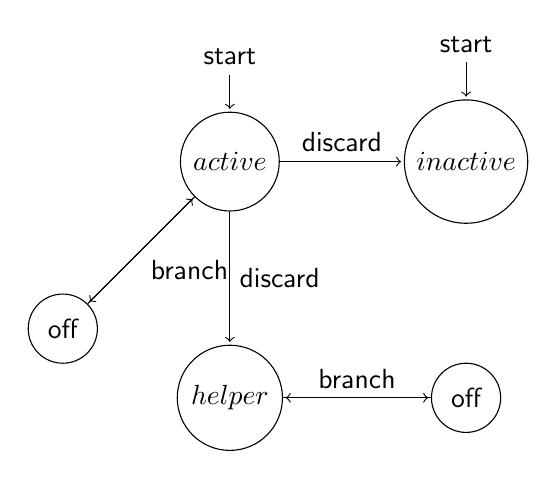
\begin{tikzpicture}[shorten >=1pt,node distance=3cm,auto, squarednode/.style={rectangle,minimum size=7mm}]
  \node[squarednode,state,initial above] (active) {$active$};
  \node[squarednode,state,initial above] (inactive)[right of=active] {$inactive$};
  \node[squarednode,state] (helper)[below of=active] {$helper$};
  \node[squarednode,state] (off1)[below left of=active] {off};
  \node[squarednode,state] (off2)[right of=helper] {off};


  \path[->] (active) edge node {discard} (inactive);
  \path[->] (active) edge node {discard} (helper);
  \path[->] (active) edge node {branch} (off1);
  \path[->] (off1) edge node {} (active);

  \path[->] (helper) edge node {branch} (off2);
  \path[->] (off2) edge node {} (helper);
\end{tikzpicture}

\Sub{\acrshort{spmd} Execution Model}{Intro.Model.Exec}

\p A runtime implementation shall provide an implementation-defined mechanism
for defining a \gls{dispatch}. A runtime shall manage hardware resources and
schedule execution to conform to the behaviors defined in this specification in
an implementation-defined way. A runtime implementation may sort the
\gls{threadgroup}s of a \gls{dispatch} into \gls{wave}s in an
implementation-defined way. During execution no guarantees are made that all
\gls{lane}s in a \gls{wave} are actively executing.

\p \gls{wave}, \gls{quad}, and \gls{threadgroup} operations require execution
synchronization of applicable active and helper \gls{lane}s as defined by the
individual operation.

\Sub{Optimization Restrictions}{Intro.Model.Restrictions}

\p An optimizing compiler may not optimize code generation such that it changes
the behavior of a well-formed program except in the presence of
\textit{implementation-defined} or \textit{unspecified} behavior.

\p The presence of \gls{wave}, \gls{quad}, or \gls{threadgroup} operations
may further limit the valid transformations of a program. Specifically, control
flow operations which result in changing which \gls{lane}s, \gls{quad}s, or
\gls{wave}s are actively executing are illegal in the presence of cooperative
operations if the optimization alters the behavior of the program.

\Sec{\acrshort{hlsl} Memory Models}{Intro.Memory}

\p Memory accesses for \gls{sm} 5.0 and earlier operate on 128-bit slots aligned
on 128-bit boundaries. This optimized for the common case in early shaders where
data being processed on the GPU was usually 4-element vectors of 32-bit data
types.

\p On modern hardware memory access restrictions are loosened, and reads of
32-bit multiples are supported starting with \gls{sm} 5.1 and reads of 16-bit
multiples are supported with \gls{sm} 6.0. \gls{sm} features are fully
documented in the \gls{dx} Specifications, and this document will not attempt to
elaborate further.

\Sub{Memory Spaces}{Intro.Memory.Spaces}

\p \acrshort{hlsl} programs manipulate data stored in four distinct memory
spaces: thread, threadgroup, device and constant.

\SubSub{Thread Memory}{Intro.Memory.Spaces.Thread}

\p Thread memory is local to the \gls{lane}. It is the default memory space used to
store local variables. Thread memory cannot be directly read from other threads
without the use of intrinsics to synchronize execution and memory.

\SubSub{\gls{threadgroup} Memory}{Intro.Memory.Spaces.Group}

\p \gls{threadgroup} memory is denoted in \acrshort{hlsl} with the
\texttt{groupshared} keyword. The underlying memory for any declaration
annotated with \texttt{groupshared} is shared across an entire
\gls{threadgroup}. Reads and writes to \gls{threadgroup} Memory, may occur in
any order except as restricted by synchronization intrinsics or other memory
annotations.

\SubSub{Device Memory}{Intro.Memory.Spaces.Device}

\p Device memory is memory available to all \gls{lane}s executing on the device.
This memory may be read or written to by multiple \gls{threadgroup}s that are
executing concurrently. Reads and writes to device memory may occur in any order
except as restricted by synchronization intrinsics or other memory annotations.
Some device memory may be visible to the host. Device memory that is visible to
the host may have additional synchronization concerns for host visibility.

\SubSub{Constant Memory}{Intro.Memory.Spaces.Constant}

\p Constant memory is similar to device memory in that it is available to all
\gls{lane}s executing on the device. Constant memory is read-only, and an
implementation can assume that constant memory is immutable and cannot change
during execution.

\Sub{Memory Spaces}{Intro.Memory.Alignment}

TODO

\p The alignment requirements of an offset into device memory space is the size
 in bytes of the largest scalar type contained in the given aggregate type.


\Ch{Lexical Conventions}{Lex}

\Sec{Unit of Translation}{Lex.Translation}

\p The text of \acrshort{hlsl} programs is collected in \textit{source} and
\textit{header} files. The distinction between source and header files is social
and not technical. An implementation will construct a \textit{translation unit}
from a single source file and any included source or header files referenced via
the \texttt{\#include} preprocessing directive conforming to the \gls{isoC}
preprocessor specification.

\p An implementation may implicitly include additional sources as required to
expose the \acrshort{hlsl} library functionality as defined in (\ref{Runtime}).

\Sec{Phases of Translation}{Lex.Phases}

\p \acrshort{hlsl} inherits the phases of translation from \gls{isoCPP}, with
minor alterations, specifically the removal of support for trigraph and digraph
sequences. Below is a description of the phases.

\begin{enumerate}
  \item Source files are characters that are mapped to the basic source
  character set in an implementation-defined manner.
  \item Any sequence of backslash (\texttt{\textbackslash}) immediately followed
  by a new line is deleted, resulting in splicing lines together.
  \item Tokenization occurs and comments are isolated. If a source file ends in
  a partial comment or preprocessor token the program is ill-formed and a
  diagnostic shall be issued. Each comment block shall be treated as a single
  white-space character.
  \item Preprocessing directives are executed, macros are expanded,
  \texttt{pragma} and other unary operator expressions are executed. Processing
  of \texttt{\#include} directives results in all preceding steps being executed
  on the resolved file, and can continue recursively. Finally all preprocessing
  directives are removed from the source.
  \item Character and string literal specifiers are converted into the
  appropriate character set for the execution environment.
  \item Adjacent string literal tokens are concatenated.
  \item White-space is no longer significant. Syntactic and semantic analysis
  occurs translating the whole translation unit into an implementation-defined
  representation.
  \item The translation unit is processed to determine required instantiations,
  the definitions of the required instantiations are located, and the
  translation and instantiation units are merged. The program is ill-formed if
  any required instantiation cannot be located or fails during instantiation.
  \item External references are resolved, library references linked, and all
  translation output is collected into a single output.
\end{enumerate}

\Sec{Character Sets}{Lex.CharSet}

\p The \textit{basic source character set} is a subset of the ASCII character set.
The table below lists the valid characters and their ASCII values:

\begin{center}
  \begin{tabular}{|| c | c | c ||}
    \hline
    Hex ASCII Value & Character Name & Glyph or C Escape Sequence \\
    \hline
    0x09 & Horizontal Tab & \texttt{\textbackslash t} \\
    0x0A & Line Feed & \texttt{\textbackslash n} \\
    0x0D & Carriage Return & \texttt{\textbackslash r} \\
    0x20 & Space & \\
    0x21 & Exclamation Mark & \texttt{!}\\
    0x22 & Quotation Mark & \texttt{"}\\
    0x23 & Number Sign & \texttt{\#}\\
    0x25 & Percent Sign & \texttt{\%}\\
    0x26 & Ampersand & \texttt{\&}\\
    0x27 & Apostrophe & \texttt{'}\\
    0x28 & Left Parenthesis & \texttt{(}\\
    0x29 & Right Parenthesis & \texttt{)}\\
    0x2A & Asterisk & \texttt{*}\\
    0x2B & Plus Sign & \texttt{+}\\
    0x2C & Comma & \texttt{,}\\
    0x2D & Hyphen-Minus & \texttt{-}\\
    0x2E & Full Stop & \texttt{.}\\
    0x2F & Solidus & \texttt{/}\\
    0x30 .. 0x39 & Digit Zero .. Nine & \texttt{0 1 2 3 4 5 6 7 8 9}\\
    0x3A & Colon & \texttt{:}\\
    0x3B & Semicolon & \texttt{;}\\
    0x3C & Less-than Sign & \texttt{<}\\
    0x3D & Equals Sign & \texttt{=}\\
    0x3E & Greater-than Sign & \texttt{>}\\
    0x3F & Question Mark & \texttt{?}\\
    0x41 .. 0x5A & Latin Capital Letter A .. Z &
        \texttt{A B C D E F G H I J K L M}\\
    & & \texttt{N O P Q R S T U V W X Y Z}\\
    0x5B & Left Square Bracket & \texttt{[}\\
    0x5C & Reverse Solidus & \texttt{\textbackslash}\\
    0x5D & Right Square Bracket & \texttt{[}\\
    0x5E & Circumflex Accent & \texttt{\textasciicircum}\\
    0x5F & Underscore & \texttt{\_}\\
    0x61 .. 0x7A & Latin Small Letter a .. z &
        \texttt{a b c d e f g h i j k l m}\\
    & & \texttt{n o p q r s t u v w x y z}\\
    0x7B & Left Curly Bracket & \texttt{\{}\\
    0x7C & Vertical Line & \texttt{|}\\
    0x7D & Right Curly Bracket & \texttt{\}}\\
    \hline
  \end{tabular}
\end{center}

\p An implementation may allow source files to be written in alternate
\textit{extended character sets} as long as that set is a superset of the
\textit{basic character set}. The \textit{translation character set} is an
\textit{extended character set} or the \textit{basic character set} as chosen by
the implementation.

\Sec{Preprocessing Tokens}{Lex.PPTokens}

\begin{grammar}
  \define{preprocessing-token}\br
  header-name\br
  identifier\br
  pp-number\br
  character-literal\br
  string-literal\br
  preprocessing-op-or-punc\br
  \textnormal{each non-whitespace character from the \textit{translation
  character set} that cannot be one of the above}
\end{grammar}\footnote{The preprocessor is inherited from C++ 11 with no
grammar extensions. It is specified here only for completeness.}

\p Each preprocessing token that is converted to a token shall have the lexical
form of a keyword, an identifier, a constant, a string literal or an operator or
punctuator.

\p Preprocessing tokens are the minimal lexical elements of the language during
translation phases 3 through 6 (\ref{Lex.Phases}). Preprocessing tokens can be
separated by whitespace in the form of comments, white space characters, or
both. White space may appear within a preprocessing token only as part of a
header name or between the quotation characters in a character constant or
string literal.

\p Header name preprocessing tokens are only recognized within
\texttt{\#include} preprocessing directives, \texttt{\_\_has\_include} expressions,
and implementation-defined locations within \texttt{\#pragma} directives. In
those contexts, a sequence of characters that could be either a header name or a
string literal is recognized as a header name.

\Sec{Tokens}{Lex.Tokens}

\begin{grammar}
  \define{token}\br
  identifier\br
  keyword\br
  literal\br
  operator-or-punctuator
\end{grammar}

\p There are five kinds of tokens: identifiers, keywords, literals, and
operators or punctuators. All whitespace characters and comments are ignored
except as they separate tokens.

\Sec{Comments}{Lex.Comments}

\p The characters \texttt{/*} start a comment which terminates with the
characters \texttt{*/}. The characters \texttt{//} start a comment
which terminates at the next new line.

\Sec{Header Names}{Lex.Headers}

\begin{grammar}
  \define{header-name}\br
  \texttt{<} h-char-sequence \texttt{>}\br
  \texttt{"} q-char-sequence \texttt{"}

  \define{h-char-sequence}\br
  h-char\br
  h-char-sequence h-char

  \define{h-char}\br
  \textnormal{any character in the \textit{translation character set} except
  newline or \texttt{>}}

  \define{q-char-sequence}\br
  q-char\br
  q-char-sequence q-char

  \define{q-char}\br
  \textnormal{any character in the \textit{translation character set} except
  newline or \texttt{"}}
\end{grammar}

\p Character sequences in header names are mapped to header files or external
source file names in an implementation defined way.

\Sec{Preprocessing numbers}{Lex.PPNumber}

\begin{grammar}
  \define{pp-number}\br
  digit\br
  \texttt{.} digit\br
  pp-number \texttt{'} digit\br
  pp-number \texttt{'} non-digit\br
  pp-number \texttt{e} sign\br
  pp-number \texttt{E} sign\br
  pp-number \texttt{p} sign\br
  pp-number \texttt{P} sign\br
  pp-number \texttt{.}
\end{grammar}

\p Preprocessing numbers begin with a digit or period (\texttt{.}), and may be
followed by valid identifier characters and floating point literal suffixes
(\texttt{e+}, \texttt{e-}, \texttt{E+}, \texttt{E-}, \texttt{p+}, \texttt{p-},
\texttt{P+}, and \texttt{P-}). Preprocessing number tokens lexically include all
\textit{integer-literal} and \textit{floating-literal} tokens.

\p Preprocessing numbers do not have types or values. Types and values are
assigned to \textit{integer-literal}, \textit{floating-literal}, and
\textit{vector-literal} tokens on successful conversion from preprocessing
numbers.

\p A preprocessing number cannot end in a period (\texttt{.}) if the immediate
next token is a \textit{scalar-element-sequence} (\ref{Lex.Literal.Vector}). In
this situation the \textit{pp-number} token is truncated to end before the
period\footnote{This grammar formulation is not context-free and requires an
LL(2) parser.}.

%\Sec{Identifiers}{Lex.Ident}

%\Sec{Keywords}{Lex.Keywords}

%\Sec{Operators and Punctuators}{Lex.Operators}

\Sec{Literals}{Lex.Literals}

\Sub{Literal Classifications}{Lex.Literal.Kinds}

\begin{grammar}
  \define{literal}\br
  integer-literal\br
  character-literal\br
  floating-literal\br
  string-literal\br
  boolean-literal\br
  vector-literal
\end{grammar}

\Sub{Integer Literals}{Lex.Literal.Int}

\begin{grammar}
  \define{integer-literal}\br
  decimal-literal \opt{integer-suffix}\br
  octal-literal \opt{integer-suffix}\br
  hexadecimal-literal \opt{integer-suffix}\br

  \define{decimal-literal}\br
  nonzero-digit\br
  decimal-literal digit\br

  \define{octal-literal}
  \terminal{0}\br
  octal-literal octal-digit\br

  \define{hexadecimal-literal}\br
  \terminal{0x} hexadecimal-digit\br
  \terminal{0X} hexadecimal-digit\br
  hexadecimal-literal hexadecimal-digit\br

  \define{nonzero-digit} \textnormal{one of}\br
  \terminal{1 2 3 4 5 6 7 8 9}\br

  \define{octal-digit} \textnormal{one of}\br
  \terminal{0 1 2 3 4 5 6 7}\br

  \define{hexadecimal-digit} \textnormal{one of}\br
  \terminal{0 1 2 3 4 5 6 7 8 9}\br
  \terminal{a b c d e f}\br
  \terminal{A B C D E F}\br

  \define{integer-suffix}\br
  unsigned-suffix \opt{long-suffix}\br
  long-suffix \opt{unsigned-suffix}\br

  \define{unsigned-suffix} \textnormal{one of}\br
  \terminal{u U}\br

  \define{long-suffix} \textnormal{one of}\br
  \terminal{l L}
\end{grammar}

\p An \textit{integer literal} is an optional base prefix, a sequence of digits
in the appropriate base, and an optional type suffix. An integer literal shall
not contain a period or exponent specifier.

\p The type of an integer literal is the first of the corresponding list in the
table below in which its value can be represented\footnote{This behavior matches
\gls{isoC} but is reduced in scope because HLSL has fewer data types.}.

\begin{center}
  \begin{tabular}{|| c | c | c ||}
    \hline
    Suffix & Decimal constant & Octal or hexadecimal constant \\
    \hline
    \hline
    none & \texttt{int32\_t} & \texttt{int32\_t} \\
         & \texttt{int64\_t} & \texttt{uint32\_t} \\
         &         & \texttt{int64\_t} \\
         &         & \texttt{uint64\_t} \\
    \hline
    \texttt{u} or \texttt{U} & \texttt{uint32\_t} & \texttt{uint32\_t} \\
                             & \texttt{uint64\_t} & \texttt{uint64\_t} \\
    \hline
    \texttt{l} or \texttt{L} & \texttt{int64\_t} & \texttt{int64\_t} \\
                             &  & \texttt{uint64\_t} \\
    \hline
    Both \texttt{u} or \texttt{U} & \texttt{uint64\_t} & \texttt{uint64\_t} \\
    and \texttt{l} or \texttt{L}  &  &  \\
    \hline
  \end{tabular}
\end{center}

\p If the specified value of an integer literal cannot be represented by any
type in the corresponding list, the integer literal has no type and the program
is ill-formed.

\p An implementation may support the integer suffixes \texttt{ll} and
\texttt{ull} as equivalent to \texttt{l} and \texttt{ul} respectively.

%\Sub{Character Literals}{Lex.Literal.Char}

\Sub{Floating-point Literals}{Lex.Literal.Float}

\begin{grammar}
  \define{floating-literal}\br
  fractional-constant \opt{exponent-part} \opt{floating-suffix}\br
  digit-sequence exponent-part \opt{floating-suffx}\br
  \define{fractional-constant}\br
  \opt{digit-sequence} \texttt{.} digit-sequence\br
  digit-sequence \texttt{.}\br
  \define{exponent-part}\br
  \texttt{e} \opt{sign} digit-sequence\br
  \texttt{E} \opt{sign} digit-sequence\br
  \define{sign} \textnormal{one of}\br
  \texttt{+} \texttt{-}\br
  \define{digit-sequence}\br
  digit\br
  digit-sequence digit
  \define{floating-suffix} \textnormal{one of}
  \texttt{h} \texttt{f} \texttt{l} \texttt{H} \texttt{F} \texttt{L}
\end{grammar}

\p A floating literal is written either as a \textit{fractional-constant} with
an optional \textit{exponent-part} and optional \textit{floating-suffix}, or as
an integer \textit{digit-sequence} with a required \textit{exponent-part} and
optional \textit{floating-suffix}.

\p The type of a floating literal is \texttt{float}, unless explicitly specified
by a suffix. The suffixes \texttt{h} and \texttt{H} specify \texttt{half}, the
suffixes \texttt{f} and \texttt{F} specify \texttt{float}, and the suffixes
\texttt{l} and \texttt{L} specify \texttt{double}.\footnote{This substantially
deviates from the implementations in \acrshort{fxc} and \acrshort{dxc}, but is
consistent with the
\href{https://learn.microsoft.com/en-us/windows/win32/direct3dhlsl/dx-graphics-hlsl-appendix-grammar\#floating-point-numbers}
{official documentation} and the behavior of GLSL. It is also
substantially simpler to implement and more regular than the existing
behaviors.} If a value specified in the source is not in the range of
representable values for its type, the program is ill-formed.

%\Sub{String Literals}{Lex.Literal.String}

%\Sub{Boolean Literals}{Lex.Literal.Bool}

\Sub{Vector Literals}{Lex.Literal.Vector}

\begin{grammar}
  \define{vector-literal}\br
  integer-literal \texttt{.} scalar-element-sequence\br
  floating-literal \texttt{.} scalar-element-sequence

  \define{scalar-element-sequence}\br
  scalar-element-sequence-x\br
  scalar-element-sequence-r

  \define{scalar-element-sequence-x}\br
  \texttt{x}\br
  scalar-element-sequence-x \texttt{x}

  \define{scalar-element-sequence-r}\br
  \texttt{r}\br
  scalar-element-sequence-r \texttt{r}
\end{grammar}

\p A \textit{vector-literal} is an \textit{integer-literal} or
\textit{floating-point} literal followed by a period (\texttt{.}) and a
\textit{scalar-element-sequence}.

\p A \textit{scalar-element-sequence} is a \textit{vector-swizzle-sequence}
where only the first vector element accessor is valid (\texttt{x} or
\texttt{r}). A \textit{scalar-element-sequence} is equivalent to a vector splat
conversion performed on the \textit{integer-literal} or
\textit{floating-literal} value (\ref{Conv.vsplat}).


\Ch{Basic Concepts}{Basic}

\begin{note}
  \p HLSL inherits a significant portion of its language semantics from C and C++.
  Some of this is a result of intentional adoption of syntax early in the development
  of the language and some a side-effect of the Clang-based implementation of DXC.

  \p This chapter includes a lot of definitions that are inherited from C and C++.
  Some are identical to C or C++, others are slightly different. HLSL is neither
  a subset nor a superset of C or C++, and cannot be simply described in terms
  of C or C++. This specification includes all necessary definitions for clarity.
\end{note}

\Sec{Preamble}{Basic.preamble}

\p An \textit{entity} is a value, object, function, enumerator, type, class
member, bit-field, template, template specialization, namespace, or pack.

\p A \textit{name} is a use of an \textit{identifier} (\ref{Expr.Primary.ID}),
\textit{operator-function-id} (\ref{Overload.operator}),
\textit{conversion-function-id} (\ref{Classes.Conversions}),
or \textit{template-id} (\ref{Template}) that denotes any entity or
\textit{label} (\ref{Stmt.Label}).

\p Every name that denotes an entity is introduced by a \textit{declaration}.
Every name that denotes a label is introduced by a \textit{labeled statement}
(\ref{Stmt.Label})\footnote{HLSL does not have \texttt{goto}, and labeled
statements are only valid within \texttt{switch} statements.}.

\p A \textit{variable} is introduced by the declaration of a reference other
than a non-static data member of an object. The variable's name denotes the
reference or object.

\p Whenever a name is encountered it is necessary to determine if the name
denotes an entity that is a type or template. The process for determining if a
name refers to a type or template is called \textit{name lookup}.

\p Two names are the same name if:
\begin{itemize}
\item they are identifiers comprised of the same character sequence, or
\item they are operator-function-ids formed with the same operator, or
\item they are conversion-function-ids formed with the same type, or
\item they are template-ids that refer to the same class or function.
\end{itemize}

\p \begin{note}
  This section matches \gls{isoCPP} section \textbf{[basic]} except for the
  exclusion of \texttt{goto} and \textit{literal operators}.
\end{note}

\Sec{Declarations and definitions}{Basic.Decl}

\p A declaration (\ref{Decl}) may introduce one or more names into a translation
unit or redeclare names introduced by previous declarations. If a declaration
introduces names, it specifies the interpretation and attributes of these names.
A declaration may also have effects such as:
\begin{itemize}
\item verifying a static assertion (\ref{Decl}),
\item use of attributes (\ref{Decl}), and
\item controlling template instantiation (\ref{Template.Inst}).
\end{itemize}

\p A declaration is a \textit{definition} unless:
\begin{itemize}
\item it declares a function without specifying the function's body
(\ref{Decl.Function}),
\item it is a parameter declaration in a function declaration that does not
specify the function's body (\ref{Decl.Function}),
\item it is a global or namespace member declaration without the \texttt{static}
specifier\footnote{Global variable declarations are implicitly constant and
external in HLSL.},
\item it declares a static data member in a class definition,
\item it is a class name declaration,
\item it is a template parameter,
\item it is a \texttt{typedef} declaration (\ref{Decl}),
\item it is an \textit{alias-declaration} (\ref{Decl}),
\item it is a \textit{using-declaration} (\ref{Decl}),
\item it is a \textit{static\_assert-declaration} (\ref{Decl}),
\item it is an \textit{empty-declaration} (\ref{Decl}),
\item or a \textit{using-directive} (\ref{Decl}).
\end{itemize}

\p The two examples below are adapted from \gls{isoCPP} \textbf{[basic.def]}. All
but one of the following are definitions:
\begin{HLSL}
int f(int x) { return x+1; } // defines f and x
struct S {int a;int b;};     // defines S, S::a, and S::b
struct X {                   // defines X
  int x;                     // defines non-static member x
  static int y;              // declares static data member y
};
int X::y = 1;                // defines X::y
enum { up, down };           // defines up and down
namespace N {                // defines N
int d;                       // declares N::d
static int i;                // defines N::i
}
\end{HLSL}

\p All of the following are declarations:
\begin{HLSL}
int a;                       // declares a
const int c;                 // declares c
X anX;                       // declares anX
int f(int);                  // declares f
struct S;                    // declares S
typedef int Int;             // declares Int
using N::d;                  // declares d
using Float = float;         // declares Float
cbuffer CB {                 // does not declare CB
  int z;                     // declares z
}
tbuffer TB {                 // does not declare TB
  int w;                     // declares w
}
\end{HLSL}

\Sec{One-Definition Rule}{Basic.ODR}

\p The \gls{isoCPP} \textit{One-definition rule} is adopted as defined in
\gls{isoCPP} \textbf{[basic.def.odr]}.

\Sec{Scope}{Basic.Scope}

\Sec{Name Lookup}{Basic.Lookup}

\Sec{Program and linkage}{Basic.Linkage}

\p A translation unit (\ref{Lex.Translation}) is comprised of a sequence of
declarations:

\begin{grammar}
  \define{translation-unit}\br
  \opt{declaration-sequence}
\end{grammar}

\p A \textit{program} is one or more translation units \textit{linked} together.
A program built from a single translation unit, bypassing a linking step is
called \textit{freestanding}.

\p A program is said to be \textit{fully linked}, when it contains no
\textit{unresolved external} declarations, and all \textit{exported}
declarations are entry point declarations (\ref{Basic.Start}). A program is said
to be \textit{partially linked}, when it contains at least one unresolved
external declaration or at least one exported declaration that is not an entry
point.

\p An implementation may generate programs as fully linked or partially linked
as requested by the user, and a runtime may allow fully linked or partially
linked programs as the implementation allows.

\p A name has \textit{linkage} if it can refer to the same entity as a name
introduced by a declaration in another scope. If a variable, function, or
another entity with the same name is declared in several scopes, but does not
have sufficient \textit{linkage}, then several instances of the entity are
generated.

\begin{itemize}
\item A name with \textit{no linkage} may not be referred to by names from
any other scope.
\item A name with \textit{internal linkage} may be referred to by names
from other scopes within the same translation unit.
\item A name with \textit{external linkage} may be referred to by names from
other scopes within the same translation unit, and by names from scopes of other
translation units.
\item A name with \textit{program linkage} may be referred to by names from
other scopes within the same translation unit, by names from scopes of other
translation units, by names from scopes of other programs, and by a runtime
implementation.
\end{itemize}

\p When merging translation units through linking or generating a freestanding
program only names with program linkage must be retained in the final program.

\Sub{Program Linkage}{Basic.Linkage.Program}

\p Entities with \textit{program linkage} can be referred to from other
partially linked programs or a runtime implementation.

\p The following entities have program linkage:
\begin{itemize}
  \item entry point functions (\ref{Basic.Start})
  \item functions marked with \texttt{export} keyword (\ref{Decl.Export})
  \item declarations contained within an \textit{export-declaration-group} (\ref{Decl.Export})
\end{itemize}

\Sub{External Linkage}{Basic.Linkage.External}

\p Entities with \textit{external linkage} can be referred to from the scopes in
the other translation units and enable linking between them.

\p The following entities in HLSL have \textit{external linkage}:
\begin{itemize}
  \item global variables that are not marked \texttt{static} or
  \texttt{groupshared} \footnote{These are not really linked with other
  translation units but rather their values are loaded indirectly based on
  cbuffer mapping.}
  \item static data members of classes or template classes
\end{itemize}

\p Linkage of functions (including template functions) that are not entry points
or marked with \texttt{export} keyword is implementation dependent. \footnote{In
DXC today functions that are not entry points or exported have \textit{internal
linkage} by default. This can be overriden by \texttt{-default-linkage} compiler
option.}

\Sub{Internal Linkage}{Basic.Linkage.Internal}

\p Entities with \textit{internal linkage} can be referred to from all scopes in
the current translation unit.

\p The following entities in HLSL have \textit{internal linkage}:
\begin{itemize}
  \item global variables marked as \texttt{static} or \texttt{groupshared}
  \item all entities declared in an unnamed namespace or a namespace within an
  unnamed namespace
  \item enumerations
  \item classes or template classes, their member functions, and nested classes
  and enumerations
\end{itemize}

\Sub{No Linkage}{Basic.Linkage.NoLinkage}

\p An entity with \textit{no linkage} can be referred to only from the scope it
is in.

\p Any of the following entites declared at function scope or block scopes
derived from function scope have no linkage:
\begin{itemize}
  \item local variables
  \item local classes and their member functions
  \item other entities declared at function scope or block scopes derived from
  function scope that such as typedefs, enumerations, and enumerators
\end{itemize}

\Sec{Start}{Basic.Start}

\p A fully linked program shall contain one or more global functions, which are
the designated starting points for the program. These global functions are
called \textit{entry points}, because they denote the location where execution
inside the program begins.

\p Entry point functions have different requirements based on the target runtime
and execution mode (\ref{Basic.Start.Mode}).

\p Parameters to entry functions and entry function return types must be of
scalar, vector, or non-intangible class type (\ref{Basic.types}). Scalar and
vector parameters and return types must be annotated with semantic annotations
(\ref{Decl.Attr.Semantic}). Class type input and output parameters must have all
fields annotated with semantic annotations.

\Sub{Execution Mode}{Basic.Start.Mode}

\p A runtime may define a set of execution modes in an implementation defined
way. Each execution mode will have a set of implementation defined rules which
restrict available language functionality as appropriate for the execution mode.

\Sec{Types}{Basic.types}

\p The \textit{object representation} of an object of type \texttt{T} is the
sequence of \textit{N} bytes taken up by the object of type \texttt{T}, where
\textit{N} equals \texttt{sizeof(T)}\footnote{\texttt{sizeof(T)} returns the
size of the object as-if it's stored in device memory, and determining the size
if it's stored in another memory space is not possible.}. The \textit{object
representation} of an object may be different based on the \textit{memory space}
it is stored in (\ref{Intro.Memory.Spaces}).

\p The \textit{value representation} of an object is the set of bits that hold
the value of type \texttt{T}. Bits in the object representation that are not
part of the value representation are \textit{padding bits}.

\p An \textit{object type} is a type that is not a function type, not a
reference type, and not a void type.

\p A \textit{class type} is a data type declared with either the \texttt{class}
or \texttt{struct} keywords (\ref{Classes}). A class type \texttt{T} may be
declared as incomplete at one point in a translation unit via a \textit{forward
declaration}, and complete later with a full definition. The type \texttt{T} is
the same type throughout the translation unit.

\p There are special implementation-defined types such as \textit{handle types},
which fall into a category of \textit{standard intangible types}. Intangible
types are types that have no defined object representation or value
representation, as such the size is unknown at compile time. Usage restrictions
for objects of intangible type are documented in \ref{Basic.types.intangible}.
% Note: The above definition is likely incomplete, and it is unclear if minimum
% precision types should be intangible.

\p A class type \texttt{T} is an \textit{intangible class type} if it contains
a base class or members of intangible class type, standard intangible type,
or arrays of such types. Standard intangible types and intangible class types
are collectively called \textit{intangible types}(\ref{Intangible}).

\p An object type is an \textit{incomplete type} if the compiler lacks
sufficient information to determine the size of an object of type \texttt{T},
and it is not an intangible type. It is a \textit{complete type} if the compiler
has sufficient information to determine the size of an object of type
\texttt{T}, or if the type is known to be an intangible type. An object may not
be defined to have an \textit{incomplete} type.

\p Arithmetic types (\ref{Basic.types.arithmetic}), enumeration types, and
\textit{cv-qualified} versions of these types are collectively called
\textit{scalar types}.

\p Vectors of scalar types declared with the built-in \texttt{vector<T,N>}
template are \textit{vector types}. Vector lengths must be between 1 and 4 (i.e.
\( 1 \leq N \leq 4 \) ).

\p Matrices of scalar types declared with the built-in \texttt{matrix<T,N,M>}
template are \textit{matrix types}. Matrix dimensions, \texttt{N} and
\texttt{M}, must be between 1 and 4 (i.e. \( 1 \leq N \leq 4 \) ).

\Sub{Arithmetic Types}{Basic.types.arithmetic}

\p There are three \textit{standard signed integer types}: \texttt{int16\_t},
\texttt{int32\_t}, and \texttt{int64\_t}. Each of the signed integer types is
explicitly named for the size in bits of the type's object representation. There
is also the type alias \texttt{int} which is an alias of \texttt{int32\_t}.
There is one \textit{minimum precision signed integer type}: \texttt{min16int}.
The minimum precision signed integer type is named for the required minimum
value representation size in bits. The object representation of
\texttt{min16int} is \texttt{int}. The standard signed integer types and minimum
precision signed integer type are collectively called \textit{signed integer
types}.

\p There are three \textit{standard unsigned integer types}: \texttt{uint16\_t},
\texttt{uint32\_t}, and \texttt{uint64\_t}. Each of the unsigned integer types
is explicitly named for the size in bits of the type's object representation.
There is also the type alias \texttt{uint} which is an alias of
\texttt{uint32\_t}. There is one \textit{minimum precision unsigned integer
type}: \texttt{min16uint}. The minimum precision unsigned integer type is named
for the required minimum value representation size in bits. The object
representation of \texttt{min16uint} is \texttt{uint}. The standard unsigned
integer types and minimum precision unsigned integer type are collectively
called \textit{unsigned integer types}.

\p The minimum precision signed integer types and minimum precision unsigned
integer types are collectively called \textit{minimum precision integer types}.
The standard signed integer types and standard unsigned integer types are
collectively called \textit{standard integer types}. The signed integer types
and unsigned integer types are collectively called \textit{integer types}.
Integer types inherit the object representation of integers defined in
\glsdesc{isoC23}\footnote{C23 adopts two's compliment as the object
representation for integer types.}. Integer types shall satisfy the constraints
defined in \glsdesc{isoCPP}, section \textbf{basic.fundamental}.

\p There are three \textit{standard floating point types}: \texttt{half},
\texttt{float}, and \texttt{double}. The \texttt{float} type is a 32-bit
floating point type. The \texttt{double} type is a 64-bit floating point type.
Both the \texttt{float} and \texttt{double} types have object representations as
defined in \gls{IEEE754}. The \texttt{half} type may be either 16-bit or 32-bit
as controlled by implementation defined compiler settings. If \texttt{half} is
32-bit it will have an object representation as defined in \gls{IEEE754},
otherwise it will have an object representation matching the \textbf{binary16}
format defined in \gls{IEEE754}\footnote{IEEE-754 only defines a binary encoding
for 16-bit floating point values, it does not fully specify the behavior of such
types.}. There is one \textit{minimum precision floating point type}:
\texttt{min16float}. The minimum precision floating point type is named for the
required minimum value representation size in bits. The object representation of
\texttt{min16float} is \texttt{float}\footnote{This means when stored to memory
objects of type \texttt{min16float} are stored as \textbf{binary32} as defined
in \gls{IEEE754}.}. The standard floating point types and minimum precision
floating point type are collectively called \textit{floating point types}.

\p Integer and floating point types are collectively called \textit{arithmetic
types}.

\p The \texttt{void} type is inherited from \gls{isoCPP}, which defines it as
having an empty set of values and being an incomplete type that can never be
completed. The \texttt{void} type is used to signify the return type of a
function that returns no value. Any expression can be explicitly converted to
\texttt{void}.

\Sub{Scalarized Type Compatability}{Basic.types.scalarized}

\p All types \texttt{T} have a \textit{scalarized representation}, \(SR(T)\),
which is a list of one or more types representing each scalar element of
\texttt{T}.

\p Scalarized representations are determined as follows:
\begin{itemize}
\item The scalarized representation of an array \texttt{T[n]} is \(SR(T_0), ..
SR(T_n)\).

\item The scalarized representation of a vector \texttt{vector<T,n>} is \(T_0,
.. T_n\).

\item The scalarized representation of a matrix \texttt{matrix<T,n, m>} is
\(T_0, .. T_{n \times m}\).

\item The scalarized representation of a class type \texttt{T}, \(SR(T)\) is
computed recursively as \(SR(T::base), SR(T::_0), .. SR(T::_n)\) where
\texttt(T::base) is \texttt{T}'s base class if it has one, and \(T::_n\)
represents the \textit{n} non-static members of \texttt{T}.

\item The scalarized representation for an enumeration type is the underlying
arithmetic type.

\item The scalarized representation for arithmetic, intangible types, and any other
type \texttt{T} is \(T\).
\end{itemize}

\p Two types \textit{cv1} \texttt{T1} and \textit{cv2} \texttt{T2} are
\textit{scalar-layout-compatible types} if \texttt{T1} and \texttt{T2} are the same
type or if the sequence of types defined by the scalar representation \(SR(T1)\)
and scalar representation \(SR(T2)\) are identical.

\Sub{Usage of Intangible Types}{Basic.types.intangible}

\p The following usage restrictions apply to intangible types:
\begin{itemize}

\item Instances of objects of intangible type may only be declared in the Thread
address space (\ref{Intro.Memory.Spaces}).

\item An object of intangible type may not be loaded or stored to any address
space other than the Thread address space
(\ref{Intro.Memory.Spaces}).\footnote{DXC supports storing objects that contain
resources in cbuffer declarations, but it does so by hoisting the resource
declaration out to the global scope.}

\item An object of intangible type may not be a parameter or return type of a
function with program linkage or external linkage (\ref{Basic.Linkage.Program}
and \ref{Basic.Linkage.External}).
\end{itemize}

\Sec{Lvalues and rvalues}{Basic.lval}

\p Expressions are classified by the type(s) of values they produce. The valid
types of values produced by expressions are:

\begin{enumerate}
  \item An \textit{lvalue} represents a function or object.
  \item An \textit{rvalue} represents a temporary object.
  \item An \textit{xvalue} (expiring value) represents an object near the end
  of its lifetime.
  \item A \textit{cxvalue} (casted expiring value) is an \textit{xvalue}
  which, on expiration, assigns its value to a bound \textit{lvalue}.
  \item A \textit{glvalue} is an \textit{lvalue}, \textit{xvalue}, or
  \textit{cxvalue}.
  \item A \textit{prvalue} is an \textit{rvalue} that is not an \textit{xvalue}.
\end{enumerate}


\Ch{Standard Conversions}{Conv}

\p \acrshort{hlsl} inherits standard conversions similar to \gls{isoCPP}. This
chapter enumerates the full set of conversions. A \textit{standard conversion
sequence} is a sequence of standard conversions in the following
order:
\begin{enumerate}
  \item Zero or one conversion of either lvalue-to-rvalue, or array-to-pointer.
  \item Zero or one conversion of either integral conversion, floating point
  conversion, floating point-integral conversion, or boolean conversion,
  derived-to-base-lvalue, or flat conversion\footnote{This differs from C++ with
  the addition of flat conversion.}.
  \item Zero or one conversion of scalar-vector splat, or vector/matrix
  truncation. \footnote{C++ does not support dimension altering conversions for
  scalar, vector or matrix types.}.
  \item Zero or one qualification conversion.
\end{enumerate}

Standard conversion sequences are applied to expressions, if necessary, to
convert it to a required destination type.

\Sec{Lvalue-to-rvalue conversion}{Conv.lval}

\p A glvalue of a non-function type \texttt{T} can be converted to a prvalue.
The program is ill-formed if \texttt{T} is an incomplete type. If the glvalue
refers to an object that is not of type \texttt{T} and is not an object of a
type derived from \texttt{T}, the program is ill-formed. If the glvalue refers to
an object that is uninitialized, the behavior is undefined. Otherwise the
prvalue is of type \texttt{T}.

\p If the glvalue refers to an array of type \texttt{T}, the prvalue will refer
to a copy of the array, not memory referred to by the glvalue.

\Sec{Array-to-pointer conversion}{Conv.array}

\p An lvalue or rvalue of type \texttt{T[]} (unsized array), can be converted to
a prvalue of type pointer to \texttt{T}\footnote{\acrshort{hlsl} does not
support grammar for specifying pointer or reference types, however they are used
in the type system and must be described in language
rules.}\footnote{Array-to-pointer conversion of constant sized arrays is not
supported.}.

\Sec{Integral promotion}{Conv.ipromote}

\p An integral promotion is a conversion of:
\begin{itemize}
  \item a glvalue of integer type other than \texttt{bool} to a cxvalue of
  integer type of higher conversion rank, or
  \item a conversion of a prvalue of integer type other than bool to a prvalue
  of integer type of higher conversion rank, or
  \item a conversion of a glvalue of type \texttt{bool} to a cxvalue of integer
  type, or
  \item a conversion of a prvalue of type \texttt{bool} to a prvalue of integer
  type.
\end{itemize}

\p Integer conversion ranks are defined in section \ref{Conv.rank.int}.

\p A conversion is only a promotion if the destination type can represent all of
the values of the source type.

\Sec{Floating point promotion}{Conv.fppromote}

\p A glvalue of a floating point type can be converted to a cxvalue of a
floating point type of higher conversion rank, or a prvalue of a floating point
type can be converted to a prvalue of a floating point type of higher conversion
rank.

\p Floating point conversion ranks are defined in section \ref{Conf.rank.float}.

\Sec{Integral conversion}{Conv.iconv}

\p A glvalue of an integer type can be converted to a cxvalue of any other
non-enumeration integer type. A prvalue of an integer type can be converted to a
prvalue of any other integer type.

\p If the destination type is unsigned, integer conversion maintains the bit pattern
of the source value in the destination type truncating or extending the value to
the destination type.

\p If the destination type is signed, the value is unchanged if the destination
type can represent the source value. If the destination type cannot represent
the source value, the result is implementation-defined.

\p If the source type is \texttt{bool}, the values \texttt{true} and
\texttt{false} are converted to one and zero respectively.

\Sec{Floating point conversion}{Conv.fconv}

\p A glvalue of a floating point type can be converted to a cxvalue of any other
floating point type. A prvalue of a floating point type can be converted to a
prvalue of any other floating point type.

\p If the source value can be exactly represented in the destination type, the
conversion produces the exact representation of the source value. If the source
value cannot be exactly represented, the conversion to a best-approximation of
the source value is implementation defined.

\Sec{Floating point-integral conversion}{Conv.fpint}

\p A glvalue of floating point type can be converted to a cxvalue of integer
type. A prvalue of floating point type can be converted to a prvalue of
integer type. Conversion of floating point values to integer values truncates by
discarding the fractional value. The behavior is undefined if the truncated
value cannot be represented in the destination type.

\p A glvalue of integer type can be converted to a cxvalue of floating point
type. A prvalue of integer type can be converted to a prvalue of floating
point type. If the destination type can exactly represent the source value, the
result is the exact value. If the destination type cannot exactly represent the
source value, the conversion to a best-approximation of the source value is
implementation defined.

\Sec{Boolean conversion}{Conv.bool}

\p A glvalue of arithmetic type can be converted to a cxvalue of boolean type. A
prvalue of arithmetic or unscoped enumeration type can be converted to a prvalue
of boolean type. A zero value is converted to \texttt{false}; all other values
are converted to \texttt{true}.

\Sec{Flat conversion}{Conv.flat}

\p There is a flattened order of subobjects for an aggregate, \texttt{A},
\texttt{A$^\prime$}, as described in section \ref{Decl.Init.Agg}.  A prvalue of an aggregate,
\texttt{A}, can be flat converted to a prvalue of an aggregate, \texttt{B}, whose flattened
form is \texttt{B$^\prime$}, if the following conditions are true: 
\begin{itemize}
\item The length of \texttt{A$^\prime$}, \texttt{N}, is greater than or equal to the
length of \texttt{B$^\prime$}, \texttt{M}.
\item For every index \texttt{I} from \texttt{0} to \texttt{M-1}, there exists an
implicit conversion from \texttt{A$^\prime$[I]} to \texttt{B$^\prime$[I]}.
\end{itemize}

\p A glvalue of type \texttt{T[N]} can be converted to a cxvalue of type \texttt{T}.

%{This is true if N is >= M but if N = M then there isnt really a cast}
\p A glvalue of type \texttt{T[N]} can be converted to a cxvalue of type \texttt{T[M]},
if \texttt{N} is greater than \texttt{M}.

\p A glvalue of type \texttt{T[N]} can be converted to a cxvalue of type
\texttt{vector<T,M>}, if \texttt{N} is greater than or equal to \texttt{M}.

\p A glvalue of type \texttt{vector<T,N>} can be converted to a cxvalue of
type \texttt{T[M]}, if \texttt{N} is greater than or equal to \texttt{M}.

\Sec{Vector splat conversion}{Conv.vsplat}

\p A glvalue of type \texttt{T} can be converted to a cxvalue of type
\texttt{vector<T,x>} or a prvalue of type \texttt{T} can be converted to a
prvalue of type \texttt{vector<T,x>}. The destination value is the source value
replicated into each element of the destination.

\p A glvalue of type \texttt{T} can be converted to a cxvalue of type
\texttt{matrix<T,x,y>} or a prvalue of type \texttt{T} can be converted to a
prvalue of type \texttt{matrix<T,x,y>}. The destination value is the source
value replicated into each element of the destination.

\p A prvalue of type \texttt{vector<T,1>} can be converted
to a prvalue of type \texttt{vector<T,x>}. The destination value is the value in
the source vector replicated into each element of the destination.

\Sec{Array and Class splat conversion}{Conv.asplat}

\p A prvalue of type \texttt{T} can be converted to a
prvalue of type \texttt{struct S}, if there are valid conversions from
\texttt{T} to each \texttt{U} in flattened \texttt{S}, see section
\ref{Decl.init.Agg} for description of a flattened ordering. The destination
value is the source value \texttt{T} replicated into each element of the
flattened \texttt{S}.

\p A prvalue of type \texttt{vector<T,1>} can be converted to a
prvalue of type \texttt{struct S}, if there are valid conversions from
\texttt{T} to each \texttt{U} in flattened \texttt{S}. The destination value is
the value in the source vector replicated into each element of the flattened
\texttt{S}.

\p A prvalue of type \texttt{T} can be converted to a
prvalue of type \texttt{U[N]}, if there are valid conversions from
\texttt{T} to each \texttt{V} in flattened \texttt{U}. The destination value
is the source value \texttt{T} replicated into each element of the flattened
\texttt{U[N]}.

\p A prvalue of type \texttt{vector<T,1>} can be converted to a
prvalue of type \texttt{U[N]}, if there are valid conversions from
\texttt{T} to each \texttt{V} in flattened \texttt{U}. The destination value
is the value in the source vector replicated into each element of the flattened
\texttt{U[N]}.

\Sec{Vector and matrix truncation conversion}{Conv.vtrunc}

\p A prvalue of type \texttt{vector<T,x>} can be converted to a prvalue of type:
\begin{itemize}
\item \texttt{vector<T,y>} only if \( y < x \), or
\item \texttt{T}
\end{itemize}

\p The resulting value of vector truncation is comprised of elements \( [0..y)
\), dropping elements \( [y..x) \).

\p A prvalue of type \texttt{matrix<T,x,y>} can be converted to a prvalue of
type:
\begin{itemize}
  \item \texttt{matrix<T,z,w>} only if \( x \geq z \) and \(y \geq w \),
  \item \texttt{vector<T,z>} only if \( x \geq z \), or
  \item \texttt{T}.
\end{itemize}

\p Matrix truncation is performed on each row and column dimension separately.
The resulting value is comprised of vectors \( [0..z) \) which are each
separately comprised of elements \( [0..w) \). Trailing vectors and elements are
dropped.

\p Reducing the dimension of a vector to one (\texttt{vector<T,1>}), can produce
either a single element vector or a scalar of type \texttt{T}. Reducing the
rows of a matrix to one (\texttt{matrix<T,x,1>}), can produce either a single
row matrix, a vector of type \texttt{vector<T,x>}, or a scalar of type
\texttt{T}.

\Sec{Component-wise conversions}{Conv.cwise}

\p A glvalue of type \texttt{vector<T,x>} can be converted to a prvalue of type
\texttt{vector<V,x>}, or a prvalue of type \texttt{vector<T,x>} can be converted
to a prvalue of type \texttt{vector<V,x>}. The source value is converted by
performing the appropriate conversion of each element of type \texttt{T} to an
element of type \texttt{V} following the rules for standard conversions
in chapter \ref{Conv}.

\p A glvalue of type \texttt{matrix<T,x,y>} can be converted to a prvalue of
type \texttt{matrix<V,x,y>}, or a prvalue of type \texttt{matrix<T,x,y>} can be
converted to a prvalue of type \texttt{matrix<V,x,y>}. The source value is
converted by performing the appropriate conversion of each element of type
\texttt{T} to an element of type \texttt{V} following the rules for standard
conversions in chapter \ref{Conv}.

\Sec{Qualification conversion}{Conv.qual}

A prvalue of type "\textit{cv1} \texttt{T}" can be converted to a prvalue of type
"\textit{cv2} \texttt{T}" if type "\textit{cv2} \texttt{T}" is more cv-qualified
than "\textit{cv1} \texttt{T}".

\Sec{Conversion Rank}{Conv.rank}

\p Every integer and floating point type have defined conversion ranks. These
conversion ranks are used to differentiate between \textit{promotions} and other
conversions (see: \ref{Conv.iprom} and \ref{Conv.fpprom}).

\Sub{Integer Conversion Rank}{Conv.rank.int}

\begin{itemize}
  \item  No two signed integer types shall have the same conversion rank even if
  they have the same representation.
  \item The rank of a signed integer type shall be greater than the rank of any
  signed integer type with a smaller size.
  \item The rank of any unsigned integer type shall equal the rank of the
  corresponding signed integer type.
  \item The rank of \texttt{bool} shall be less than the rank of all other
  standard integer types.
  \item The rank of a minimum precision integer type shall be less than the rank
  of any other minimum precision integer type with a larger minimum value
  representation size.
  \item The rank of a minimum precision integer type shall be less than the rank
  of all standard integer types.
  \item For all integer types \texttt{T1}, \texttt{T2}, and \texttt{T3}: if
  \texttt{T1} has greater rank than \texttt{T2} and \texttt{T2} has greater rank
  than \texttt{T3}, then \texttt{T1} shall have greater rank than \texttt{T3}.
\end{itemize}

\Sub{Floating Point Conversion Rank}{Conv.rank.float}

\begin{itemize}
  \item The rank \texttt{half} shall be greater than the rank of \texttt{min16float}.
  \item The rank \texttt{float} shall be greater than the rank of \texttt{half}.
  \item The rank \texttt{double} shall be greater than the rank of \texttt{float}.
  \item For all floating point types \texttt{T1}, \texttt{T2}, and \texttt{T3}:
  if \texttt{T1} has greater rank than \texttt{T2} and \texttt{T2} has greater
  rank than \texttt{T3}, then \texttt{T1} shall have greater rank than
  \texttt{T3}.
\end{itemize}

\Ch{Expressions}{Expr}

\p This chapter defines the formulations of expressions and the behavior of
operators when they are not overloaded. Only member operators may be
overloaded\footnote{This will change in the future, but this document assumes
current behavior.}. Operator overloading does not alter the rules for operators
defined by this standard.

\p An expression may also be an \textit{unevaluated operand} when it appears in
some contexts. An \textit{unevaluated operand} is a expression which is not
evaluated in the program\footnote{The operand to \texttt{sizeof(...)} is a good
example of an \textit{unevaluated operand}. In the code \texttt{sizeof(Foo())},
the call to \texttt{Foo()} is never evaluated in the program.}.

\p Whenever a \textit{glvalue} appears in an expression that expects a
\textit{prvalue}, a standard conversion sequence is applied based on the rules
in \ref{Conv}.

\Sec{Usual Arithmetic Conversions}{Expr.conv}
\p Binary operators for arithmetic and enumeration type require that both
operands are of a common type. When the types do not match the \textit{usual
arithmetic conversions} are applied to yield a common type. When \textit{usual
arithmetic conversions} are applied to vector operands they behave as
component-wise conversions (\ref{Conv.cwise}). The \textit{usual arithmetic
conversions} are:

\begin{itemize}
  \item If either operand is of scoped enumeration type no conversion is
  performed, and the expression is ill-formed if the types do not match.
  \item If either operand is a \texttt{vector<T,X>}, vector truncation or scalar
  extension is performed with the following rules:
  \begin{itemize}
    \item If both vectors are of the same length, no dimension conversion is
    required.
    \item If one operand is a vector and the other operand is a scalar, the
    scalar is extended to a vector via a Splat conversion (\ref{Conv.vsplat}) to
    match the length of the vector.
    \item Otherwise, if both operands are vectors of different lengths, the
    vector of longer length is truncated to match the length of the shorter
    vector (\ref{Conv.vtrunc}).
  \end{itemize}
  \item If either operand is of type \texttt{double} or \texttt{vector<double,
  X>}, the other operator shall be converted to match.
  \item Otherwise, if either operand is of type \texttt{float} or \texttt{vector<float,
  X>}, the other operand shall be converted to match.
  \item Otherwise, if either operand is of type \texttt{half} or \texttt{vector<half, X>},
  the other operand shall be converted to match.
  \item Otherwise, integer promotions are performed on each scalar or vector
  operand following the appropriate scalar or component-wise conversion
  (\ref{Conv}).
  \begin{itemize}
    \item If both operands are scalar or vector elements of signed or unsigned
    types, the operand of lesser integer conversion rank shall be converted to
    the type of the operand with greater rank.
    \item Otherwise, if both the operand of unsigned scalar or vector element
    type is of greater rank than the operand of signed scalar or vector element
    type, the signed operand is converted to the type of the unsigned operand.
    \item Otherwise, if the operand of signed scalar or vector element type is
    able to represent all values of the operand of unsigned scalar or vector
    element type, the unsigned operand is converted to the type of the signed
    operand.
    \item Otherwise, both operands are converted to a scalar or vector type of
    the unsigned integer type corresponding to the type of the operand with
    signed integer scalar or vector element type.
  \end{itemize}
\end{itemize}

\Sec{Primary Expressions}{Expr.Primary}

\begin{grammar}
  \define{primary-expression}\br
  literal\br
  \keyword{this}\br
  \terminal{(} expression \terminal{)}\br
  id-expression\br
\end{grammar}

\Sub{Literals}{Expr.Primary.Literal}

\p The type of a \textit{literal} is determined based on the grammar forms
specified in \ref{Lex.Literal.Kinds}.

\Sub{This}{Expr.Primary.This}

\p The keyword \keyword{this} names a reference to the implicit object of
non-static member functions. The \keyword{this} parameter is always a
\textit{prvalue} of non-\textit{cv-qualified}type.
\footnote{
  \href{https://github.com/microsoft/hlsl-specs/blob/main/proposals/0007-const-instance-methods.md}
  {HLSL Specs Proposal 0007} proposes adopting C++-like syntax and semantics for
  \textit{cv-qualified} \keyword{this} references.}

\p A \keyword{this} expression shall not appear outside the declaration of a
non-static member function.

\Sub{Parenthesis}{Expr.Primary.Paren}

\p An expression (\textit{E}) enclosed in parenthesis has the same type, result
and value category as \textit{E} without the enclosing parenthesis. A
parenthesized expression may be used in the same contexts with the same meaning
as the same non-parenthesized expression.

\Sub{Names}{Expr.Primary.ID}

\begin{note}
  The grammar and behaviors of this section are almost identical to C/C++ with
  some subtractions (notably lambdas and destructors).
\end{note}

\begin{grammar}
  \define{id-expression}\br
  unqualified-id\br
  qualified-id
\end{grammar}

\SubSub{Unqualified Identifiers}{Expr.Primary.ID.Unqual}

\begin{grammar}
  \define{unqualified-id}\br
  identifier\br
  operator-function-id\br
  conversion-function-id\br
  template-id\br
\end{grammar}

\SubSub{Qualified Identifiers}{Expr.Primary.ID.Qual}

\begin{grammar}
  \define{qualified-id}\br
  nested-name-specifier \opt{\keyword{template}} unqualified-id\br

  \define{nested-name-specifier}\br
  \terminal{::}\br
  type-name \terminal{::}\br
  namespace-name \terminal{::}\br
  nested-name-specifier identifier \terminal{::}\br
  nested-name-specifier \opt{\keyword{template}} simple-template-id \terminal{::}
\end{grammar}

\Sec{Postfix Expressions}{Expr.Post}

\begin{grammar}
  \define{postfix-expression}\br
  primary-expression\br
  % The [] characters on the two lines below should be inside \terminal, however
  % pandoc doesn't seem to like that.
  postfix-expression [ expression ]\br
  postfix-expression [ braced-init-list ]\br %
  postfix-expression \terminal{(} \opt{expression-list} \terminal{)}\br
  simple-type-specifier \terminal{(} \opt{expression-list} \terminal{)}\br
  typename-specifier \terminal{(} \opt{expression} \terminal{)}\br
  simple-type-specifier braced-init-list\br
  typename-specifier braced-init-list\br
  postfix-expression \terminal{.} \opt{\terminal{template}} id-expression\br
  postfix-expression \terminal{.} vector-swizzle-component-sequence\br
  postfix-expression \terminal{++}\br
  postfix-expression \terminal{--}
\end{grammar}

\Sec{Subscript}{Expr.Post.Subscript}

\p A \textit{postfix-expression} followed by an expression in square brackets
(\texttt{[ ]}) is a subscript expression. In an array subscript expression of
the form \texttt{E1[E2]}, \texttt{E1} must either be a variable of array,
vector, or matrix of \texttt{T[]}, or an object of type \texttt{T} where
\texttt{T} provides an overloaded implementation of \texttt{operator[]}
(\ref{Overload}).\footnote{HLSL does not support the base address of a subscript
operator being the expression inside the braces, which is valid in C and C++.}

\p If the postfix expression \texttt{E1} is of vector type, the expression
\textit{E2} must be a value of integer type. If the value is known at compile
time to be outside the range \texttt{[0, N-1]} where \texttt{N} is the number of
elements in the vector, the program is ill-formed. If the value is outside the
range at runtime, the behavior is undefined.

\Sec{Vector Swizzle}{Expr.Post.VectorSwizzle}

\begin{grammar}
  \define{vector-swizzle-component-sequence}\br
  swizzle-component-sequence-rgba\br
  swizzle-component-sequence-xyzw\br

  \define{swizzle-component-sequence-rgba}\br
  swizzle-component-rgba\br
  swizzle-component-sequence-rgba swizzle-component-rgba\br

  \define{swizzle-component-sequence-xyzw}\br
  swizzle-component-xyzw\br
  swizzle-component-sequence-xyzw swizzle-component-xyzw\br

  \define{swizzle-component-rgba}\br
  \terminal{r}\br
  \terminal{g}\br
  \terminal{b}\br
  \terminal{a}\br

  \define{swizzle-component-xyzw}\br
  \terminal{x}\br
  \terminal{y}\br
  \terminal{z}\br
  \terminal{w}
\end{grammar}

\p A \textit{postfix-expression} followed by a dot (\texttt{.}) and a sequence
of one or more \textit{swizzle-components} is a postfix expression. The
postfix expression before the dot is evaluated and must be of vector type. If
the postfix expression before the dot is an lvalue, the swizzle expression may
produce either an lvalue or a prvalue; otherwise it produces a prvalue.

\p A \textit{swizzle-component-sequence} is a sequence of one or more swizzle
components of either the \textit{swizzle-component-rgba} or
\textit{swizzle-component-xyzw} forms; the two forms may not be mixed in the
same \textit{swizzle-component-sequence}. If the postfix expression before the
dot is an lvalue and the \textit{swizzle-component-sequence} contains no
repeated components, the swizzle expression is an lvalue; otherwise it is a
prvalue.

\p Swizzle components map to elements of the vector in the following way:

\begin{center}
  \begin{tabular}{|| c | c | c ||}
    \hline
    Element Index & RGBA component & XYZW component \\
    \hline
    0 & r & x \\
    1 & g & y \\
    2 & b & z \\
    3 & a & w \\
    \hline
  \end{tabular}
\end{center}

\p A program is ill-formed if any component in the \textit{swizzle-component-sequence}
refers to an element index that is out of range of the vector type of the
postfix expression before the dot.

\Sec{Function Calls}{Expr.Post.Call}

\p A function call may be an \textit{ordinary function}, or a \textit{member
function}. In a function call to an \textit{ordinary function}, the
\textit{postfix-expression} must be an lvalue that refers to a function. In a
function call to a \textit{member function}, the \textit{postfix-expression}
will be an implicit or explicit class member access whose \textit{id-expression}
is a member function name.

\p When a function is called, each parameter shall be initialized with its
corresponding argument. The order in which parameters are initialized is
unspecified. \footnote{Today in DXC targeting DXIL matches the Microsoft C++ ABI
and evaluates argument expressions right-to-left, while SPIR-V generation
matches the Itanium ABI evaluating parameters left-to-right. There are good
arguments for unifying these behaviors, and arguments for keeping them
different.}

\p If the function is a non-static member function the \texttt{this} argument
shall be initialized to a reference to the object of the call as if casted by an
explicit cast expression to an lvalue reference of the type that the function is
declared as a member of.

\p Parameters are either \textit{input parameters}, \textit{output parameters},
or \textit{input/output parameters} as denoted in the called function's
declaration (\ref{Decl.Function}). For all types of parameters the argument
expressions are evaluated before the function call occurs.

\p \textit{Input parameters} are passed by-value into a function. If an argument
to an \textit{input parameter} is of constant-sized array type, the array is
copied to a temporary and the temporary value is converted to an address via
array-to-pointer decay. If an argument is an unsized array type, the array
lvalue directly decays via array-to-pointer decay. \footnote{This results in
\textit{input} parameters of unsized arrays being modifiable by a function.}

\p Arguments to \textit{output} and \textit{input/output parameters} must be
lvalues. \textit{Output parameters} are not initialized prior to the call; they
are passed as an uninitialized cxvalue (\ref{Basic.lval}). An \textit{output
parameter} is only initialized explicitly inside the called function. It is
undefined behavior to not explicitly initialize an \textit{output parameter}
before returning from the function in which it is defined. The cxvalue created
from an argument to an \textit{input/output parameter} is initialized through
copy-initialization from the lvalue argument expression. Overload resolution
shall occur on argument initialization as if the expression \texttt{T Param =
Arg} were evaluated. In both cases, the cxvalue shall have the type of the
parameter and the argument can be converted to that type through implicit or
explicit conversion.

\p If an argument to an \textit{output} or \textit{input/output parameter} is a
constant sized array, the array is copied to a temporary cxvalue following the
same rules for any other data type. If an argument to an \textit{output} or
\textit{input/output parameter} is an unsized array type, the array lvalue
directly decays via array-to-pointer decay. An argument of a constant sized
array of type \texttt{T[N]} can be converted to a cxvalue of an unsized array
of type \texttt{T[]} through array to pointer decay. An unsized array of type
\texttt{T[]}, cannot be implicitly converted to a a constant sized array of type
\texttt{T[N]}.

\p On expiration of the cxvalue, the value is assigned back to the argument
lvalue expression using a resolved assignment expression as if the expression
\texttt{Arg = Param} were written\footnote{The argument expression is not
re-evaluated after the call, so any side effects of the call occur only before
the call.}. The argument expression must be of a type or able to convert to a
type that has defined copy-initialization to and assignment from the parameter
type. The lifetime of the cxvalue begins at argument expression evaluation, and
ends after the function returns. A cxvalue argument is passed by-address to the
caller.

\p If the lvalue passed to an \textit{output} or \textit{input/output parameter}
does not alias any other parameter passed to that function, an implementation
may avoid the creation of excess temporaries by passing the address of the
lvalue instead of creating the cxvalue.

\p When a function is called, any parameter of object type must have completely
defined type, and any parameter of array of object type must have completely
defined element type.\footnote{HLSL \textit{output} and \textit{input/output
parameters} are passed by value, so they must also have complete type.} The
lifetime of a parameter ends on return of the function in which it is
defined.\footnote{As stated above cxvalue parameters are passed-by-address, so
the expiring parameter is the reference to the address, not the cxvalue. The
cxvalue expires in the caller.} Initialization and destruction of each
parameter occurs within the context of the calling function.

\p The value of a function call is the value returned by the called function.

\p A function call is an lvalue if the result type is an lvalue reference type;
otherwise it is a prvalue.

\p If a function call is a prvalue of object type, the type of the prvalue must
be complete.

\Ch{Statements}{Stmt}
\Sec{Label Statements}{Stmt.Label}
\Sec{Attributes}{Stmt.Attr}
\Sub{Unroll Attribute}{Stmt.Attr.Unroll}
The \texttt{[unroll]} and \texttt{[unroll(n)]} attribute qualifiers can be used
 to specify that a loop (\texttt{for}, \texttt{while} and \texttt{do while} 
loops) can be unrolled. This attribute qualifier can be used to specify full 
unrolling or partial unrolling by a specified amount. This is a compiler hint 
and the compiler may ignore this directive.

\texttt{n} is the loop unrolling factor and must be a positive integral compile time 
constant expression. If n is not specified, the compiler determines the 
unrolling factor for the loop. This attribute is not compatible with the \texttt{[loop]}
 attribute.

Note:  The \texttt{[unroll]} attribute  must appear immediately before the loop
 to be affected.

\subsubsection{Unroll Examples}{Stmt.Attr.Unroll.Examples}
\begin{itemize}
\item  Requests the compiler to unroll the above \texttt{for} loop by a factor 
of 2.
\begin{HLSL}
[unroll(2)]
int sum = 0;
for (int i=0; i<32; i++)
    sum += i;
\end{HLSL}
\item In this example, the compiler will determine how much to unroll the loop.
\begin{HLSL}
int i = 0;
[unroll]
do {
    ...
    i++;
} while(i < 32);
\end{HLSL}
\item Below is an  examples of \textbf{\emph{invalid}} usage of 
\texttt{[unroll(n)]} because n is not positive
\begin{HLSL}
[unroll(-1)]
while (...)
{
    ...
}
\end{HLSL}
\item This example is \textbf{\emph{invalid}} because the \texttt{[unroll]} 
attribute is used on a non-loop construct
\begin{HLSL}
[unroll]
if (...)
{
    ...
}
\end{HLSL}
\item The below example is \textbf{\emph{invalid}} because the loop unroll 
factor is not a compile-time constant expression.
\begin{HLSL}
    int x;
    [unroll(x)]
    for (int i=0; i<x; i++)
    {
        ...
    }
\end{HLSL}
\end{itemize}
\Sub{Loop Attribute}{Stmt.Attr.Loop}
The Attribute \texttt{[loop]} tells the compiler to execute each iteration of 
the loop. In other words, its a hint to indicate a loop should not be 
unrolled. Therefore it is not compatible with the \texttt{[unroll]} attribute.

Note:  The \texttt{[loop]} attribute  must appear immediately before the loop
 to be affected.
 
\subsubsection{Loop Examples}{Stmt.Attr.Loop.Examples}
\begin{itemize}
\item  Tell the compiler to not to unroll the loop.
\begin{HLSL}
[loop]
for (int i=0; i<32; i++) {
    ...
}
\end{HLSL}
\item This example is \textbf{\emph{invalid}} because the \texttt{[loop]} 
attribute is used on a non-loop construct
\begin{HLSL}
[loop]
if (...)
{
    ...
}
\end{HLSL}
\end{itemize}
\Ch{Declarations}{Decl}
\Sec{Preamble}{Decl.Pre}
\p Declarations generally specify how names are to be interpreted. Declarations have the form
\begin{grammar}
  \define{declaration-seq}\br
  \textit{declaration}\br
  \textit{declaration-seq declaration}

  \define{declaration}\br
  \textit{name-declaration}\br
  \textit{special-declaration}\br
  \textit{empty-declaration}

  \define{name-declaration}\br
  \textit{variable-declaration}\br
  \textit{function-declaration}\br
  \textit{namespace-declaration}\br
  \textit{record-declaration}\br
  \textit{template-declaration}\br
  \textit{type-alias-declaration}\br
  ...
  
  \define{special-declaration}\br
  \textit{export-declaration-group}\br
  \textit{cbuffer-declaration-group}\br
  ...

  \define{empty-declaration} \terminal{;}
  
\end{grammar}

\Sec{Specifiers}{Decl.Spec}
\Sub{General}{Decl.Spec.General}
\p The specifiers that can be used in a declaration are
\begin{grammar}
  \define{decl-specifier}\br
  \textit{function-specifier}\br
  ...
\end{grammar}

\Sub{Function specifiers}{Decl.Spec.Fct}

\p A \textit{function-specifier} can be used only in a function declaration.

\begin{grammar}
  \define{function-specifier}\br
  \texttt{export}\br
\end{grammar}

\p The \texttt{export} specifier denotes that the function has program linkage (\ref{Basic.Linkage.Program}).

\p The \texttt{export} specifier cannot be used on functions directly or indirectly within an unnamed namespace.

\p Functions with program linkage can also be specified in \textit{export-declaration-group} (\ref{Decl.Export}).

\p If a function is declared with an \texttt{export} specifier then all redeclarations of the same function must also use the \texttt{export} specifier or be part of \textit{export-declaration-group} (\ref{Decl.Export}).

\Sec{Declarators}{Decl.Decl}
\Sec{Initializers}{Decl.Init}

\p The process of initialization described in this section applies to all
initializers regardless of the context.

\begin{grammar}
  \define{initializer}\br
  brace-or-equal-initializer\br
  \terminal{(} expression-list \terminal{)}\br

  \define{brace-or-equal-initializer}\br
  \terminal{=} initializer-clause\br
  braced-init-list\br

  \define{initializer-clause}\br
  assignment-expression\br
  braced-init-list\br

  \define{braced-init-list}\br
  \terminal{\{} initializer-list \opt{\terminal{,}} \terminal{\}}\br
  \terminal{\{} \terminal{\}}\br

  \define{initializer-list}\br
  initializer-clause\br
  initializer-list \terminal{,} initializer-clause\br
\end{grammar}

\Sub{Aggregate Initialization}{Decl.Init.Agg}

\p An \textit{aggregate} is a vector, matrix, array, or class.

\p The subobjects of an aggregate have a defined order. For vectors and arrays
the order is increasing subscript order. For matrices it is increasing subscript
order with the subscript nesting such that in the notation
\texttt{Mat[M][N]}, the ordering is \(Mat[0][0]...Mat[0][N]...
Mat[M][0]...Mat[M][N]\). For classes the order is base class, followed by member
subobjects in declaration order.

\p A \textit{flattened ordering} of subobjects can be produced by performing a
depth-first traversal of the subobjects of an object following the defined
subobject ordering.

\p Each \textit{braced initializer list} is comprised of zero or more
\textit{initializer-clause} expressions, which is either another braced
initializer list or an expression which generates a value that either is or can
be implicitly converted to an rvalue. Each assignment-expression is an object,
which may be a scalar or aggregate type. A \textit{flattened initializer
sequence} is constructed by a depth-first traversal over each
assignment-expression in an initializer-list and performing a depth-first
traversal accessing each subobject of the assignment-expression.

\p An initializer-list is a valid initializer if for each element \(E_n\) in the
target object's flattened ordering there is a corresponding initializer \(I_n\)
in the flattened initializer sequence which can be implicitly converted to the
element's type.

\p An initializer-list is invalid if the flattened initializer sequence contains
more or fewer elements than the target object's flattened ordering, or if any
initializer \(I_n\) cannot be implicitly converted to the corresponding element
\(E_n\)'s type.

\Sec{Function Definitions}{Decl.Function}
\Sec{Attributes}{Decl.Attr}
\Sub{Semantic Annotations}{Decl.Attr.Semantic}
\Sub{Entry Attributes}{Decl.Attr.Entry}

\Sec{Export Declarations}{Decl.Export}

\p One or more functions with \textit{external linkage} can be also specified in the form of

\begin{grammar}
  \define{export-declaration-group}\br
  \texttt{export} \terminal{\{} \opt{function-declaration-seq} \terminal{\}}\br

  \define{function-declaration-seq}\br
  \textit{function-declaration} \opt{function-declaration-seq}
\end{grammar}

\p The \texttt{export} specifier denotes that every \textit{function-declaration} included in \textit{function-declaration-seq} has \textit{external linkage} (\ref{Basic.Linkage.External}).

\p The \textit{export-declaration-group} declaration cannot appear directly or indirectly within an unnamed namespace.

\p Functions with \textit{external linkage} can also be declared with an \texttt{export} specifier (\ref{Decl.Spec.Fct}).

\p If a function is part of an \textit{export-declaration-group} then all redeclarations of the same function must also be part on a \textit{export-declaration-group} or be declared with an \texttt{export} specifier (\ref{Decl.Spec.Fct}).

\Ch{Overloading}{Overload}

\begin{note}
\p HLSL inherits much of its overloading behavior from C++. This chapter is
extremely similar to \gls{isoCPP} clause \textbf{[over]}. Notable differences
exist around HLSL's parameter modifier keywords, program entry points, and
overload conversion sequence ranking.
\end{note}

\p When a single name is declared with two or more different declarations in the
same scope, the name is \textit{overloaded}. A declaration that declares an
overloaded name is called an \textit{overloaded declaration}. The set of
overloaded declarations that declare the same overloaded name are that name's
\textit{overload set}.

\p Only function and template declarations can be overloaded; variable and type
declarations cannot be overloaded.

\Sec{Overloadable Declarations}{Overload.Decl}

\p This section specifies the cases in which a function declaration cannot be
overloaded. Any program that contains an invalid overload set is ill-formed.

\p In overload set is invalid if:
\begin{itemize}
  \item One or more declaration in the overload set only differ by return type.
\begin{HLSL}
int Yeet();
uint Yeet(); // ill-formed: decls differ only by return type
\end{HLSL}

  \item An overload set contains more than one member function declarations with
  the same \textit{parameter-type-list}, and one of those declarations is a
  \texttt{static} member function declaration (\ref{Classes.Static}).
\begin{HLSL}
class Doggo {
  static void pet();
  void pet();              // ill-formed: static pet has the same parameter-type-list
  void pet() const;        // ill-formed: static pet has the same parameter-type-list

  void wagTail();          // valid: no conflicting static declaration.
  void wagTail() const;    // valid: no conflicting static declaration.

  static void bark(Doggo D);
  void bark();             // valid: static bark parameter-type-list is different
  void bark() const;       // valid: static bark parameter-type-list is different
};
\end{HLSL}

  \item An overload set contains more than one entry function declaration
  (\ref{Decl.Attr.Entry}).
\begin{HLSL}
[shader("vertex")]
void VS();
void VS(int);              // valid: only one entry point.

[shader("vertex")]
void Entry();

[shader("compute")]
void Entry(int);           // ill-formed: an overload set cannot have more than one entry function
\end{HLSL}

  \item An overload set contains more than one function declaration which only
  differ in parameter declarations of equivalent types.
\begin{HLSL}
void F(int4 I);
void F(vector<int, 4> I);  // ill-formed: int4 is a type alias of vector<int, 4>
\end{HLSL}

  \item An overload set contains more than one function declaration which only
  differ in \texttt{const} specifiers.
\begin{HLSL}
void G(int);
void G(const int);         // ill-formed: redeclaration of G(int)
void G(int) {}
void G(const int) {}       // ill-formed: redefinition of G(int)
\end{HLSL}

  \item An overload set contains more than one function declaration which only
  differ in parameters mismatching \texttt{out} and \texttt{inout}.
\begin{HLSL}
void H(int);
void H(in int);            // valid: redeclaration of H(int)
void H(inout int);         // valid: overloading between in and inout is allowed

void I(in int);
void I(out int);           // valid: overloading between in and out is allowed

void J(out int);
void J(inout int);         // ill-formed: Cannot overload based on out/inout mismatch
\end{HLSL}
\end{itemize}

\Sec{Overload Resolution}{Overload.Res}

\p \textit{Overload resolution} is process by which a function call is mapped to
a the best overloaded function declaration. Overload resolution uses set of
functions called the \textit{candidate set}, and a list of expressions that
comprise the argument list for the call.

\p Overload resolution selects the function to call in the following
contexts\footnote{DXC only supports overload resolution for function calls and
invocation of operators during expressions. Clang will support all contexts
listed.}:

\begin{itemize}
  \item invocation of a function named in a function call expression;
  \item invocation of a function call operator on a class object named in
  function call syntax;
  \item invocation of the operator referenced in an expression;
  \item invocation of a user-defined conversion for copy-initialization of a
  class object;
  \item invocation of a conversion function for initialization of an object of a
  nonclass type from an expression of class type.
\end{itemize}

\p In each of these contexts a unique method is used to construct the overload
candidate set and argument expression list.

\Sub{Candidate Functions and Argument Lists}{Overload.Res.Sets}

\begin{note}
  \gls{isoCPP} goes into a lot of detail in this section about how candidate
  functions and argument lists are selected for each context where overload
  resolution is performed. HLSL matches C++ for the contexts that HLSL inherits.
  For now, this section will be left as a stub, but HLSL inherits the following
  sections from C++:
  \begin{itemize}
    \item \textbf{[over.call.func]}
    \item \textbf{[over.call.object]}
    \item \textbf{[over.match.oper]}
    \item \textbf{[over.match.copy]}
    \item \textbf{[over.match.conv]}
  \end{itemize}
\end{note}

\Sub{Viable Functions}{Overload.Res.Viable}

\p Given the candidate set and argument expressions as determined by the
relevant context (\ref{Overload.Res.Sets}), a subset of viable functions can be
selected from the candidate set.

\p A function candidate \(F(P_0 ... P_m)\) is not a viable function for a call
with argument list \(A_0 ... A_n\) if:
\begin{itemize}
  \item The function has fewer parameters than there are
  arguments in the argument list (\(m < n \)).
  \item The function has more parameters than there are arguments to the
  argument list (\(m > n \)), and function parameters \( P_{n+1} ... P_m \) do not
  all have default arguments.
  \item There is not an implicit conversion sequence that converts each argument
  \(A_i\) to the type of the corresponding parameter \(P_i\).
\end{itemize}

\Sub{Best Viable Function}{Overload.Res.Best}

\p For an overloaded call with arguments \(A_0 ... A_n\), each viable function
\(F(P_0 ... P_m)\), has a set of implicit conversion sequences \(ICS_0(F) ...
ICS_m(F)\) defining the conversion sequences for each argument \(A_i\) to the
type of parameter \(P_i\).

\p A viable function \(F\) is defined to be a better function than another
viable function \(F`\) if for all arguments \(ICS_i(F)\) is not a worse
conversion sequence than \(ICS_i(F`)\), and:
\begin{itemize}
  \item for some argument \(j\), \(ICS_j(F)\) is a better conversion than
  \(ICS_j(F`)\) or,
  \item in the context of an initialization by user-defined conversion, the
  conversion sequence from the return type of \(F\) to the destination type is a
  better conversion sequence than the return type of \(F`\) to the destination
  type or,
  \item \(F\) is a non-template function and \(F`\) is a function template
  specialization, or
  \item \(F\) and \(F`\) are both function template specializations and \(F\) is
  more specialized than \(F`\) according to function template partial ordering
  rules (\ref{Template.Func.Order}).
\end{itemize}

\p If there is one viable function that is a better function than all the other
viable functions, it is the selected function; otherwise the call is ill-formed.

\p If the resolved overload is a function with multiple declarations, and if at
least two of these declarations specify a default argument that made the
function viable, the program is ill-formed.

\begin{HLSL}
void F(int X = 1);
void F(float Y = 2.0f);

void Fn() {
  F(1);     // Okay.
  F(3.0f);  // Okay.
  F();      // Ill-formed.
}
\end{HLSL}

\Sub{Implicit Conversion Sequences}{Overload.ICS}

\p An \textit{implicit conversion sequence} is a sequence of conversions which
converts a source value to a prvalue of destination type. In overload resolution
the source value is the argument expression in a function call, and the
destination type is the type of the corresponding parameter of the function
being called.

\p When a parameter is a cxvalue an \textit{inverted implicit conversion
sequence} is required to convert the parameter type back to the argument type
for writing back to the argument expression lvalue. An inverted implicit
conversion sequence must be a well-formed implicit conversion sequence where the
source value is the implicit cxvalue of the parameter type, and the destination
type is the argument expression's lvalue type.

\p A well-formed implicit conversion sequence is either a \textit{standard
conversion sequence}, or a \textit{user-defined conversion sequence}.

\p In the following contexts an implicit conversion sequence can only be a
standard conversion sequence:
\begin{itemize}
  \item Argument conversion for a user-defined conversion function.
  \item Copying a temporary for class copy-initialization.
  \item When passing an initializer-list as a single argument.
  \item Copy-initialization of a class by user-defined conversion.
\end{itemize}

\p An implicit conversion sequence models a copy-initialization unless it is an
inverted implicit conversion sequence when it models an assignment. Any
difference in top-level cv-qualification is handled by the copy-initialization
or assignment, and does not constitute a conversion\footnote{"Top-level"
cv-qualification refers to the qualification of the value. This means an
parameter of type \texttt{T} can be initialized by a argument of type
\texttt{const T}. This does not mean that a parameter of type \texttt{inout T}
can be initialized with a argument of type \texttt{const T} because there is no
valid inverted conversion system to assign back to a value of type \texttt{const
T}.}.

\p When the source value type and the destination type are the same, the
implicit conversion sequence is an \textit{identity conversion}, which signifies
no conversion.

\p Only standard conversion sequences that do not create temporary objects are
valid for implicit object parameters or left operand to assignment operators.

\p If no sequence of conversions can be found to convert a source value to the
destination type, an implicit conversion sequence cannot be formed.

\p If several different sequences of conversions exist that convert the source
value to the destination type, the implicit conversion sequence is defined to be
the unique conversion sequence designated the \textit{ambiguous conversion
sequence}. For the purpose of ranking implicit conversion sequences, the
ambiguous conversion sequence is treated as a user-defined sequence that is
indistinguishable from any other user-defined conversion sequence. If overload
resolution selects a function using the ambiguous conversion sequence as the
best match for a call, the call is ill-formed.

\SubSub{Standard Conversion Sequences}{Overload.ICS.SCS}

\p The conversions that comprise a standard conversion sequence and the
composition of the sequence are defined in Chapter \ref{Conv}.

\p Each standard conversion is given a category and rank as defined in the table
below:
\begin{center}
  \begin{tabular}{|| c | c | c | c ||}
    \hline
    Conversion & Category & Rank & Reference \\
    \hline
    No conversion & Identity &  & \\ \cline{1-2}\cline{4-4}

    Lvalue-to-rvalue & & & \ref{Conv.lval} \\ \cline{4-4}
    Array-to-pointer & Lvalue Transformation & Exact Match
          & \ref{Conv.array} \\ \cline{1-2}\cline{4-4}
    Qualification & Qualification Adjustment & & \ref{Conv.qual} \\ \cline{1-4}

    Scalar splat (without conversion) & Scalar Extension & Extension
          & \ref{Conv.vsplat} \\ \cline{1-4}

    Integral promotion & &
          & \ref{Conv.iconv} \& \ref{Conv.rank.int} \\ \cline{1-1}\cline{4-4}
    Floating point promotion & Promotion & Promotion
          & \ref{Conv.fconv} \& \ref{Conv.rank.float} \\ \cline{1-1}\cline{4-4}
    Component-wise promotion &  &  & \ref{Conv.cwise} \\ \cline{1-4}

    Scalar splat promotion & Scalar Extension Promotion & Promotion Extension
          & \ref{Conv.vsplat} \\ \cline{1-4}

    Integral conversion & & & \ref{Conv.iconv} \\ \cline{1-1}\cline{4-4}
    Floating point conversion &  &  & \ref{Conv.fconv} \\ \cline{1-1}\cline{4-4}
    Floating-integral conversion & Conversion & Conversion
          & \ref{Conv.fpint} \\ \cline{1-1}\cline{4-4}
    Boolean conversion &  &  & \ref{Conv.bool} \\ \cline{1-1}\cline{4-4}
    Component-wise conversion &  &  & \ref{Conv.cwise} \\ \cline{1-4}

    Scalar splat conversion & Scalar Extension Conversion & Conversion Extension
          & \ref{Conv.vsplat} \\ \cline{1-4}

    Vector truncation (without conversion) & Dimensionality Reduction
          & Truncation & \ref{Conv.vtrunc} \\ \cline{1-4}

    Vector truncation promotion & Dimensionality Reduction Promotion
          & Promotion Truncation & \ref{Conv.vtrunc} \\ \cline{1-4}

    Vector truncation conversion & Dimensionality Reduction Conversion
          & Conversion Truncation & \ref{Conv.vtrunc} \\ \cline{1-4}
    \hline
  \end{tabular}
\end{center}

\p If a scalar splat conversion occurs in a conversion sequence where all other
conversions are \textbf{Exact Match} rank, the conversion is ranked as
\textbf{Extension}. If a scalar splat occurs in a conversion
sequence with a \textbf{Promotion} conversion, the conversion is ranked as
\textbf{Promotion Extension}. If a scalar splat occurs in a conversion
sequence with a \textbf{Conversion} conversion, the conversion is ranked as
\textbf{Conversion Extension}.

\p If a vector truncation conversion occurs in a conversion sequence where all
other conversions are \textbf{Exact Match} rank, the conversion is ranked as
\textbf{Truncation}. If a vector truncation occurs in a conversion
sequence with a \textbf{Promotion} conversion, the conversion is ranked as
\textbf{Promotion Truncation}. If a vector truncation occurs in a conversion
sequence with a \textbf{Conversion} conversion, the conversion is ranked as
\textbf{Conversion Truncation}.

\p Otherwise, the rank of a conversion sequence is determined by considering the
rank of each conversion.

\p Conversion sequence ranks are ordered from better to worse as:
\begin{enumerate}
  \item \textbf{Exact Match}
  \item \textbf{Extension}
  \item \textbf{Promotion}
  \item \textbf{Promotion Extension}
  \item \textbf{Conversion}
  \item \textbf{Conversion Extension}
  \item \textbf{Truncation}
  \item \textbf{Promotion Truncation}
  \item \textbf{Conversion Truncation}
\end{enumerate}

% TODO: Define user-defined conversion sequences. DXC doesn't actually support
% these because we don't resolve overloads for user-defined conversion
% functions, but in Clang we will. This will likely match C++ extremely close so
% it can be left to fill out later.

\SubSub{Comparing Implicit Conversion Sequences}{Overload.ICS.Comparing}

\p A partial ordering of implicit conversion sequences exists based on defining
relationships for \textit{better conversion sequence}, and \textit{better
conversion}. If an implicit conversion sequence \(ICS(f)\) is a better
conversion sequence than \(ICS(f`)\), then the inverse is also true: \(ICS(f`)\)
is a \textit{worse conversion sequence} than \(ICS(f)\). If \(ICS(f)\) is
neither better nor worse than \(ICS(f`)\), the conversion sequences are
\textit{indistinguishable conversion sequences}.

\p A standard conversion sequence is always better than a user-defined
conversion sequence.

\p Standard conversion sequences are ordered by their ranks. Two conversion
sequences with the same rank are indistinguishable unless one of the following
rules applies:

\begin{itemize}
  \item If class \texttt{B} is derived directly or indirectly from class
  \texttt{A} and class \texttt{C} is derived directly or indirectly from class
  \texttt{B},
  \begin{itemize}
    \item binding of a expression of type \texttt{C} to a cxvalue of type
    \texttt{B} is better than binding an expression of type \texttt{C} to a
    cxvalue of type \texttt{A},
    \item conversion of \texttt{C} to \texttt{B} is better than conversion or
    \texttt{C} to \texttt{A},
    \item binding of a expression of type \texttt{B} to a cxvalue of type
    \texttt{A} is better than binding an expression of type \texttt{C} to a
    cxvalue of type \texttt{A},
    \item conversion of \texttt{B} to \texttt{A} is better than conversion of
    \texttt{C} to \texttt{A}.
  \end{itemize}
\end{itemize}

\Ch{Resource Types}{Resources}

Resources are built-in intangible types representing memory with an external interface.

These take the form of Typed Buffers, Raw Buffers, Textures, and Samplers.
Buffer and Texture types can be read-only or writable.

\Sec{Typed Buffers}{Resources.tybuf}

The typed buffer class template represents a one-dimensional resource containing an array of a single given type.
Its contents are indexed by typed access to each element
Types may have their formats converted upon load.

Template types can be any type that totals or can be padded to 16 bytes.

All typed buffers can be read through subscript operators or Load methods.
Writable typed buffers can be written through subscript operators.

Where \texttt{T} can be any arithmetic type \ref{Basic.types.arithmetic}
or a vector with a maximum of four elements containing such an arithmetic type.
The total size of a single contained element must be less than 16 bytes.

Typed buffers perform format conversions on load such that the underlying data
gets converted to the destination type.

\Sec{Typed Buffers}{Resources.tybufs}

\begin{HLSL}
template <typename T = float4>
 class Buffer {
 public:
   Buffer();
   Buffer(Buffer buf);
   Buffer operator=(Buffer buf);

   void GetDimensions(out uint width) const;

   // Element access.
   T operator[](int pos) const;
   T Load(in int pos) const;
   T Load(in int pos, out uint status) const;
};


template <typename T>
 class RWBuffer : public Buffer {
 public:
   RWBuffer();
   RWBuffer(RWBuffer buf);
   RWBuffer operator=(RWBuffer buf);

   // element access
   T &operator[](int n);
};
}
\end{HLSL}

\Sub{Constructors}{Resources.tybufs.ctrs}

Read-only Buffers can be defined with explicit or implicit template parameter types.
\begin{HLSL}
  Buffer buf1;
  Buffer<> buf2;
  Buffer<float4> buf3;
\end{HLSL}
Since \texttt{float4} is the default type, all of these definitions are equivalent.

RWBuffers must be defined with explicit template parameter types.
\begin{HLSL}
  RWBuffer<float4> buf;
\end{HLSL}

When defined at global scope, typed buffers are bound to externally-defined backing stores
using the explicit binding location if provided or the implicit binding if not.

When defined at local scope, typed buffers represent local references
that can be associated with global buffers when assigned,
but must be resolvable to a unique global buffer.

\begin{HLSL}
  Buffer<int> grobuf;
  RWBuffer<int> grwbuf;
  void main() {
    Buffer<int> lrobuf = grobuf;
    RWBuffer<int> lrwbuf = grwbuf;
  }
\end{HLSL}
Buffer operands to the assignment operator must have the same element type.

\Sub{Dimensions}{Resources.tybufs.dims}

The size of a typed buffer can be retrieved using the \texttt{GetDimensions} method.
\begin{HLSL}
void GetDimensions(out uint width) const;
\end{HLSL}

This returns the full legnth, in elements of the buffer through the \texttt{width} out parameter.

\Sub{Element Access}{Resources.tybufs.access}

The contents of typed buffers can be retrieved using the \texttt{Load} methods
or the subscript operator.

\begin{HLSL}
 T Load(in int pos) const;
 T operator[](int pos) const;
\end{HLSL}

These each return the element at the given position \texttt{pos} of the type specified in the buffer definition.

An additional \texttt{Load} method returns the indicated element just as the other,
but also takes a second \texttt{status} parameter that returns information about the accessed resource.
\begin{HLSL}
 T Load(in int pos, out uint status) const;
\end{HLSL}

The \texttt{status} parameter returns an indication of whether all of the retrieved value
came from fully mapped parts of the resource.
This parameter must be passed to the built-in function \texttt{CheckAccessFullyMapped} (\ref{Resources.mapcheck})
in order to interpret it.

Writable buffers have an additional subscript operator that allows assignment to an element of the buffer.
It behaves as if it returns a reference to that element.
\begin{HLSL}
 T &operator[](int pos);
\end{HLSL}

Partial writes aren't allowed.
Assignment to individual vector elements will result in an error.

\Sec{Raw Buffer Types}{Resources.rawbufs}

Raw buffers are one-dimensional resources of arbitrary memory layout.
They are either ByteAddressBuffers or StructuredBuffers.
ByteAddressBuffers enable per-byte access to the raw data while
StructuredBuffers have an associated structure type that determines how they are
indexed. This type can be a scalar, vector, matrix, or user-defined struct.

\Sec{Byte Access Buffers}{Resources.babufs}

\begin{HLSL}
 class ByteAddressBuffer {
 public:
   ByteAddressBuffer();
   ByteAddressBuffer(ByteAddressBuffer buf);
   ByteAddressBuffer operator=(ByteAddressBuffer buf);

   void GetDimensions(out uint size) const;

   // Element access.
   uint Load(in uint byteOffset) const;
   uint2 Load2(in uint byteOffset) const;
   uint3 Load3(in uint byteOffset) const;
   uint4 Load4(in uint byteOffset) const;
   template<typename T>
   T Load(in uint byteOffset) const;

   uint Load(in uint byteOffset, out uint status) const;
   uint2 Load2(in uint byteOffset, out uint status) const;
   uint3 Load3(in uint byteOffset, out uint status) const;
   uint4 Load4(in uint byteOffset, out uint status) const;
   template<typename T>
   T Load(in uint byteOffset, out uint status) const;
};

 class RWByteAddressBuffer : public ByteAddressBuffer {
 public:
   RWByteAddressBuffer();
   RWByteAddressBuffer(RWByteAddressBuffer buf);
   RWByteAddressBuffer operator=(RWByteAddressBuffer buf);

   // Element assignment.
   void Store(in uint byteOffset, in uint value);
   void Store2(in uint byteOffset, in uint2 value);
   void Store3(in uint byteOffset, in uint3 value);
   void Store4(in uint byteOffset, in uint4 value);
   template<typename T>
   void Store(in uint byteOffset, in T value);

   // 32-bit integer atomic arithmetic/bitwise operations.
   void InterlockedAdd(in uint pos, in uint value);
   void InterlockedAdd(in uint pos, in uint value, out uint original);
   void InterlockedAnd(in uint pos, in uint value);
   void InterlockedAnd(in uint pos, in uint value, out uint original);
   void InterlockedOr(in uint pos, in uint value);
   void InterlockedOr(in uint pos, in uint value, out uint original);
   void InterlockedXor(in uint pos, in uint value);
   void InterlockedXor(in uint pos, in uint value, out uint original);

   // 32-bit integer atomic comparison operations
   void InterlockedMin(in uint pos, in int value);
   void InterlockedMin(in uint pos, in uint value);
   void InterlockedMin(in uint pos, in int value, out int original);
   void InterlockedMin(in uint pos, in uint value, out uint original);
   void InterlockedMax(in uint pos, in int value);
   void InterlockedMax(in uint pos, in uint value);
   void InterlockedMax(in uint pos, in int value, out int original);
   void InterlockedMax(in uint pos, in uint value, out uint original);

   // 32-bit integer atomic compare/exchange operations
   void InterlockedCompareStore(in uint pos, in uint compare, in uint value);
   void InterlockedExchange(in uint pos, in uint value, out uint original);
   void InterlockedCompareExchange(in uint pos, in uint compare, in uint value,
                                    out uint original);

   // 64-bit integer atomic arithmatic/bitwise operations
   void InterlockedAdd64(in uint pos, in uint64_t value);
   void InterlockedAdd64(in uint pos, in uint64_t value, out uint64_t original);
   void InterlockedAnd64(in uint pos, in uint64_t value);
   void InterlockedAnd64(in uint pos, in uint64_t value, out uint64_t original);
   void InterlockedOr64(in uint pos, in uint64_t value);
   void InterlockedOr64(in uint pos, in uint64_t value, out uint64_t original);
   void InterlockedXor64(in uint pos, in uint64_t value);
   void InterlockedXor64(in uint pos, in uint64_t value, out uint64_t original);

   // 64-bit integer atomic comparison operations
   void InterlockedMin64(in uint pos, in int64_t value);
   void InterlockedMin64(in uint pos, in int64_t value, out int64_t original);
   void InterlockedMin64(in uint pos, in uint64_t value);
   void InterlockedMin64(in uint pos, in uint64_t value, out uint64_t original);
   void InterlockedMax64(in uint pos, in int64_t value);
   void InterlockedMax64(in uint pos, in int64_t value, out int64_t original);
   void InterlockedMax64(in uint pos, in uint64_t value);
   void InterlockedMax64(in uint pos, in uint64_t value, out uint64_t original);

   // 64-bit integer atomic compare/exchange operations
   void InterlockedCompareStore64(in uint pos, in uint64_t compare, in uint64_t value);
   void InterlockedExchange64(in uint pos, in int64_t value, out int64_t original);
   void InterlockedCompareExchange64(in uint pos, in uint64_t compare,
                                      in uint64_t value, out int64_t original);

   // 32-bit float atomic compare/exchange operations
   void InterlockedCompareStoreFloatBitwise(in uint byteOffest,
                                             in float compare, in float value);
   void InterlockedExchangeFloat(in uint byteOffest, in float value,
                                  out float original);
   void InterlockedCompareExchangeFloatBitwise(in uint byteOffest,
                                                in float compare,
                                                in float value,
                                                out float original);
};
\end{HLSL}

\Sub{Constructors}{Resources.babufs.ctrs}

Since their contents are viewed as raw bytes, ByteAddressBuffers are defined without any type parameters.
\begin{HLSL}
  ByteAddressBuffer robuf;
  RWByteAddressBuffer rwbuf;
\end{HLSL}

When defined at global scope, ByteAccessBuffers are bound to externally-defined backing stores
using the explicit binding location if provided or the implicit binding if not.

When defined at local scope, ByteAccessBuffers represent local references
that can be associated with global ByteAccessBuffers when assigned,
but must be resolvable to a unique global buffer.

\begin{HLSL}
  ByteAddressBuffer grobuf;
  RWByteAddressBuffer grwbuf;
  void main() {
    ByteAddressBuffer lrobuf = grobuf;
    RWByteAddressBuffer lrwbuf = grwbuf;
  }
\end{HLSL}

\Sub{Dimensions}{Resources.babufs.dims}

The size of a ByteAddressBuffer can be retrieved using the \texttt{GetDimensions} method.
\begin{HLSL}
void GetDimensions(out uint size) const;
\end{HLSL}

This returns the full size of the buffer in bytes through the \texttt{size} out parameter.

\Sub{Element Access}{Resources.babufs.access}

The contents of ByteAddressBuffers can be retrieved using the \texttt{Load} methods.

\begin{HLSL}
 uint Load(in uint byteOffset) const;
 uint2 Load2(in uint byteOffset) const;
 uint3 Load3(in uint byteOffset) const;
 uint4 Load4(in uint byteOffset) const;
\end{HLSL}

These each return the bytes at the given position \texttt{byteOffset} in the form of one or more unsigned integers.
The \texttt{byteOffset} address is in bytes and must be a multiple of 4.
Each of the variants returns a number of bytes corresponding to the size of the uint vector returned.

An additional templated load method allows returning the bytes at the given byte offset in the form
of the type given in the template parameter. This can be a scalar, vector, matrix, or user-defined struct.

\begin{HLSL}
  template<typename T>
  T Load(in uint byteOffset) const;
\end{HLSL}

The alignment requirements of \texttt{byteOffset} for this operation is the size in bytes of the largest
scalar type contained in the given tyep \texttt{T}.

Additional \texttt{Load} methods return the same values as the others,
but also take a second \texttt{status} parameter that returns information about the accessed resource.
\begin{HLSL}
  uint Load(in uint byteOffset, out uint status) const;
  uint2 Load2(in uint byteOffset, out uint status) const;
  uint3 Load3(in uint byteOffset, out uint status) const;
  uint4 Load4(in uint byteOffset, out uint status) const;
  template<typename T>
  T Load(in uint byteOffset, out uint status) const;
\end{HLSL}

The \texttt{status} parameter returns an indication of whether all of the retrieved value
came from fully mapped parts of the resource.
This parameter must be passed to the built-in function \texttt{CheckAccessFullyMapped} (\ref{Resources.mapcheck})
in order to interpret it.

\Sub{Atomic Operations}{Resources.babufs.atomics}

RWByteAddressBuffers have a suite of atomic methods that perform the given operation
on signed or unsigned integer element data indexed by the given integer size
in a way that ensures no contention from other threads performing other operations.
Each has an overload that optionally returns the original value before the atomic operation was performed.

\begin{HLSL}
   void InterlockedAdd(in uint pos, in uint value);
   void InterlockedAdd(in uint pos, in uint value, out uint original);
   void InterlockedAnd(in uint pos, in uint value);
   void InterlockedAnd(in uint pos, in uint value, out uint original);
   void InterlockedOr(in uint pos, in uint value);
   void InterlockedOr(in uint pos, in uint value, out uint original);
   void InterlockedXor(in uint pos, in uint value);
   void InterlockedXor(in uint pos, in uint value, out uint original);
\end{HLSL}

Perform atomic addition, bitwise and, bitwise or, or bitwise exclusive or
on the element found in 32-bit integer position \texttt{pos} and the provided \texttt{value}
and stores the resulting sum in that buffer position,
optionally returning the orignal value of the buffer position through \texttt{original}

\begin{HLSL}
   void InterlockedMin(in uint pos, in int value);
   void InterlockedMin(in uint pos, in uint value);
   void InterlockedMin(in uint pos, in int value, out int original);
   void InterlockedMin(in uint pos, in uint value, out uint original);
   void InterlockedMax(in uint pos, in int value);
   void InterlockedMax(in uint pos, in uint value);
   void InterlockedMax(in uint pos, in int value, out int original);
   void InterlockedMax(in uint pos, in uint value, out uint original);
\end{HLSL}

Perform the sign-approrpriate minimum or maximum comparison of the 32-bit integer indexed by \texttt{pos}
and the provided \texttt{value} and assigns the less or greater as appropriate to that buffer position,
optionally returning the orignal value at that buffer position through \texttt{original}

\begin{HLSL}
   void InterlockedExchange(in uint pos, in uint value, out uint original);
\end{HLSL}

Performs an atomic exchange of the the 32-bit integer indexed by \texttt{pos} with
the value of \texttt{value} and returns the original value at that position through \texttt{original}.

\begin{HLSL}
   void InterlockedCompareStore(in uint pos, in uint compare, in uint value);
   void InterlockedCompareExchange(in uint pos, in uint compare, in uint value,
                                    out uint original);
\end{HLSL}

Perform an atomic exchange of or store to the the 32-bit integer indexed by \texttt{pos}
with the provided \texttt{value} if the value at that position matches the value of \texttt{compare}.
\texttt{InterlockedCompareExchange} returns the original value at that position through \texttt{original}.

\begin{HLSL}
   void InterlockedAdd64(in uint pos, in uint64_t value);
   void InterlockedAdd64(in uint pos, in uint64_t value, out uint64_t original);
   void InterlockedAnd64(in uint pos, in uint64_t value);
   void InterlockedAnd64(in uint pos, in uint64_t value, out uint64_t original);
   void InterlockedOr64(in uint pos, in uint64_t value);
   void InterlockedOr64(in uint pos, in uint64_t value, out uint64_t original);
   void InterlockedXor64(in uint pos, in uint64_t value);
   void InterlockedXor64(in uint pos, in uint64_t value, out uint64_t original);
\end{HLSL}

Performs atomic addition, bitwise and, bitwise or, or bitwise exclusive or
on the element found in 64-bit integer position \texttt{pos} and the provided \texttt{value}
and stores the resulting sum in that buffer position,
optionally returning the orignal value of the buffer position through \texttt{original}

\begin{HLSL}
   void InterlockedMin64(in uint pos, in int64_t value);
   void InterlockedMin64(in uint pos, in uint64_t value);
   void InterlockedMin64(in uint pos, in int64_t value, out int64_t original);
   void InterlockedMin64(in uint pos, in uint64_t value, out uint64_t original);
   void InterlockedMax64(in uint pos, in int64_t value);
   void InterlockedMax64(in uint pos, in uint64_t value);
   void InterlockedMax64(in uint pos, in int64_t value, out int64_t original);
   void InterlockedMax64(in uint pos, in uint64_t value, out uint64_t original);
\end{HLSL}

Performs the sign-approrpriate minimum or maximum comparison of the 64-bit integer indexed by \texttt{pos}
and the provided \texttt{value} and assigns the less or greater as appropriate to that buffer position,
optionally returning the orignal value at that buffer position through \texttt{original}

\begin{HLSL}
   void InterlockedExchange64(in uint pos, in uint64_t value, out uint64_t original);
\end{HLSL}

Performs an atomic exchange of the the 64-bit integer indexed by \texttt{pos} with
the value of \texttt{value} and returns the original value at that position through \texttt{original}.

\begin{HLSL}
   void InterlockedCompareStore64(in uint pos, in uint64_t compare,
                                   in uint64_t value);
   void InterlockedCompareExchange64(in uint pos, in uint64_t compare,
                                      in uint64_t value, out uint64_t original);
\end{HLSL}

Perform an atomic exchange of or store to the the 64-bit integer indexed by \texttt{pos}
with the provided \texttt{value} if the value at that position matches the value of \texttt{compare}.
\texttt{InterlockedCompareExchange64} returns the original value at that position through \texttt{original}.

\begin{HLSL}
   void InterlockedExchangeFloat(in uint byteOffest, in float value,
                                  out float original);
\end{HLSL}

Performs an atomic exchange of the the 32-bit float indexed by \texttt{pos} with
the value of \texttt{value} and returns the original value at that position through \texttt{original}.

\begin{HLSL}
  void InterlockedCompareStoreFloatBitwise(in uint byteOffest, in float compare,
                                            in float value);
  void InterlockedCompareExchangeFloatBitwise(in uint byteOffest,
                                               in float compare,
                                               in float value,
                                               out float original);
\end{HLSL}

Perform an atomic exchange of or store to the the 32-bit float indexed by
\texttt{pos} with the provided \texttt{value} if the value at that position
matches the value of \texttt{compare} in a bitwise comparison.
\texttt{InterlockedCompareExchangeFloatBitwise} returns the original value at
that position through \texttt{original}.

Unlike standard floating point comparisons, values will only match if the bit
representation matches which can miss some matching values that have different
bit repesantations in addition to ignoring floating point rules surrounding NaN
and infinite values.

\Sec{Structured Buffers}{Resources.stbufs}

Structured buffers are raw buffers with associated types that facilitate
indexing.
Unlike typed buffers, they perform no format conversions.
The buffer contents is treated as raw data and the casting to the given types
is done bit for bit.
Structured buffers can be defined with scalar, vector, matrix, or user-defined
struct elements.

\Sec{Structured Buffers}{Resources.stbufs}

Structured buffers can be read-only, writable, appendable, or consumable.
Writable buffers can have their elements assigned in arbitrary locations.
Append structured buffers can only have elements added to the end.
Consume structured buffers can only have elements removed from the end.

\begin{HLSL}
template <typename T>
 class StructuredBuffer {
 public:
   StructuredBuffer();
   StructuredBuffer(StructuredBuffer buf);
   StructuredBuffer operator=(StructuredBuffer buf);

   void GetDimensions(out uint count, out uint stride) const;

   // Element access.
   T operator[](int pos) const;
   T Load(in int pos) const;
   T Load(in int pos, out uint status) const;
};

 class RWStructuredBuffer {
 public:
   RWStructuredBuffer();
   RWStructuredBuffer(RWStructuredBuffer buf);
   RWStructuredBuffer operator=(RWStructuredBuffer buf);

   // Element assignment.
   T &operator[](int pos);

   // Hidden counter increment/decrement.
   uint IncrementCounter();
   uint DecrementCounter();
};

template <typename T>
 class AppendStructuredBuffer {
   AppendStructuredBuffer();
   AppendStructuredBuffer(AppendStructuredBuffer buf);
   AppendStructuredBuffer operator=(AppendStructuredBuffer buf);

   void GetDimensions(out uint count, out uint stride) const;

   void Append(in T value);
};

template <typename T>
 class ConsumeStructuredBuffer {
   ConsumeStructuredBuffer();
   ConsumeStructuredBuffer(ConsumeStructuredBuffer buf);
   ConsumeStructuredBuffer operator=(ConsumeStructuredBuffer buf);

   void GetDimensions(out uint count, out uint stride) const;

   void Consume();
};

\end{HLSL}

\Sub{Constructors}{Resources.stbufs.ctrs}

Structured buffers must be defined with explicit template parameter types.
\begin{HLSL}
  struct S {int i; float f;};
  StructuredBuffer<S> robuf1;
  StructuredBuffer<float4> robuf2;
  StructuredBuffer<float2x3> robuf3;

  RWStructuredBuffer<S> rwbuf1;
  RWStructuredBuffer<float4> rwbuf2;
  RWStructuredBuffer<float2x3> rwbuf3;

  AppendStructuredBuffer<S> apbuf1;
  AppendStructuredBuffer<float4> apbuf2;
  AppendStructuredBuffer<float2x3> apbuf3;

  ConsumeStructuredBuffer<S> cobuf1;
  ConsumeStructuredBuffer<float4> cobuf2;
  ConsumeStructuredBuffer<float2x3> cobuf3;
\end{HLSL}

When defined at global scope, structured buffers are bound to externally-defined backing stores
using the explicit binding location if provided or the implicit binding if not.

When defined at local scope, structured buffers represent local references
that can be associated with global buffers when assigned,
but must be resolvable to a unique global buffer.

\begin{HLSL}
  StructuredBuffer<int3x3> grobuf;
  RWStructuredBuffer<int3x3> grwbuf;
  AppendStructuredBuffer<int3x3> gapbuf;
  ConsumeStructuredBuffer<int3x3> gcobuf;
  void main() {
    StructuredBuffer<int3x3> lrobuf = grobuf;
    RWStructuredBuffer<int3x3> lrwbuf = grwbuf;
    AppendStructuredBuffer<int3x3> lbuf = gapbuf;
    ConsumeStructuredBuffer<int3x3> lcobuf = gcobuf;
  }
\end{HLSL}
Structured buffer operands to the assignment operator must have the same element type.

\Sub{Dimensions}{Resources.stbufs.dims}

The structure count and stride of a structured buffer can be retrieved using the \texttt{GetDimensions} method.
\begin{HLSL}
void GetDimensions(out uint count, out uint stride);
\end{HLSL}

This returns number of structured elements of the buffer through the \texttt{count} out parameter
and the size of each element in bytes through the \texttt{stride} out parameter.

\Sub{Element Access}{Resources.stbufs.access}

The contents of read-only StructuredBuffers and writable RWStructuredBuffers can be retrieved
using the \texttt{Load} methods or the subscript operator.

\begin{HLSL}
 T Load(in int pos) const;
 T operator[](int pos) const;
\end{HLSL}

These each return the element at the given position \texttt{pos} of the type specified in the buffer definition.

An additional \texttt{Load} method returns the indicated element just as the other,
but also takes a second \texttt{status} parameter that returns information about the accessed resource.
\begin{HLSL}
 T Load(in int pos, out uint status) const;
\end{HLSL}

The \texttt{status} parameter returns an indication of whether all of the retrieved value
came from fully mapped parts of the resource.
This parameter must be passed to the built-in function \texttt{CheckAccessFullyMapped} (\ref{Resources.mapcheck})
in order to interpret it.

Writable RWStructuredBuffers have an additional subscript operator that allows assignment to a structure element of the buffer.
It behaves as if it returns a reference to that element.
\begin{HLSL}
 T &operator[](int pos);
\end{HLSL}

\Sub{Counter Manipulation}{Resources.stbufs.counter}

RWStructuredBuffers may have a hidden counter that can be incremented and decremented using methods.

\begin{HLSL}
   uint IncrementCounter();
   uint DecrementCounter();
\end{HLSL}

Increment or decrements the hidden counter associated with the RWStructuredBuffer.

\Sub{Append}{Resources.stbufs.append}

AppendStructuredBuffers can only be appended to as an output stream.

\begin{HLSL}
   void Append(in T value);
\end{HLSL}

Appends the \texttt{value} of the template parameter types to the end of the AppendStructuredBuffer.
Subsequent appends will continue to add elements to the end of the buffer.

\Sub{Consume}{Resources.cnstbufs.consume}

ConsumeStructuredBuffers can only have values pulled from them as an input stream.

\begin{HLSL}
   void Consume();
\end{HLSL}

Removes and returns a value of the template parameter types from the end of the ConsumeStructuredBuffer.

\Sec{Constant Buffers}{Resources.cnbuf}

\Sec{Samplers}{Resources.samp}

\Sec{CheckAccessFullyMapped}{Resources.mapcheck}

The mapped status value returned by certain texture and buffer methods can be intrepreted by a built-in function:

\begin{HLSL}
  bool CheckAccessFullyMapped(in uint status);
\end{HLSL}

This function returns true is the value was accessed from a fully committed resource,
or from fully mapped pages of a sparse resource.
If any part of the return value was from unmapped memory, false is returned.

\Sec{Resource Binding}{Resources.binding}

Resources are bound to external memory using virtual registers within logical registers spaces.
These can be specified explicitly using attributes after the global resource declaration
or implicitly by leaving them off.

\begin{grammar}
  \define{resource-binding}\br
  \terminal{: register(} register-type bind-number \terminal{)}\br
  \terminal{: register(} register-type bind-number , \terminal{space} bind-number \terminal{)}\br
  \define{register-type} \textnormal{one of}\br
  \terminal{t u b s}\br
  \define{bind-number}\br
  digit\br
  bind-number digit\br
\end{grammar}

The register type indicates whether the binding is for a read-only (\texttt{t}), a writable (\texttt{u}),
a constant buffer (\texttt{b}), or a sampler (\texttt{s}).
The register bind number indicates the register number at which the resource variable begins.
The optional second parameter indicates the virtual register space that the register belongs to.

Sample syntax of virtual register binding attributes:
\begin{HLSL}
  Buffer<float> robuf : register(t0, space0);
  RWBuffer<float> rwbuf : register(u0, space0);
  SamplerState samp : register(s0, space0);
  cbuffer cbuf : register(b0, space0) { float f; };
\end{HLSL}

Each resource must have a unique register. Different resources cannot occupy the same register,
but read-only and writable buffers have separate namespaces and different logical register spaces have independent
sets of register numbers. Meaning the following is all allowed:
\begin{HLSL}
  Buffer<float> mybuf : register(t0, space0);
  Buffer<float> yourbuf : register(t0, space1);
  RWBuffer<float> hisbuf : register(u0, space0);
  RWBuffer<float> herbuf : register(u0, space1);
\end{HLSL}

Resource aggregates structs containing multiple resources types or arrays of resource types or structs containing one or more resource types.
When aggregate types have register annotations, they occupy the first register they specify as well as however many additional sequential registers
the aggregate requires to assign a register to each of its elements that correspond to the given register type.
Multiple register annotations can be placed on aggregates involving structs where each corresponds to a distinct
register type that will apply to all the registers of that type in the aggregate.

\begin{note}
Resource types contained in structs are only allocated registers when they are explicitly used.
This includes elements of arrays of resources as such array elements must be indexed with literals.
\end{note}

\begin{HLSL}
  // Occupies t0, t1, and t2.
  Buffer<float> fbuf[3] : register(t0, space0);
  // Occupies registers t3 - t14.
  Buffer<int4> ibuf[4][3] : register(t3, space0);
  // Occupies registers t15 and u0.
  struct {RWBuffer<int> rwbuf; Buffer buf;} sbufs : register(t15) : register(u0);
  // Occupies registers t16 - t21.
  struct {Buffer bufs[5]; Buffer buf;} robufs : register(t16);
  // Occupies registers t22-24 and u1-u2
  struct {Buffer r; RWBuffer<int> w;} bibufs[2] : register(t22) : register(u1);
\end{HLSL}

If the register binding or register space is not specified, implicit values are used.
Whenever not specified, the space defaults to \texttt{space0}.

\begin{HLSL}
  Buffer<float2> buf1 : register(t0, space0);
  Buffer<float2> buf2 : register(t1); // defaults to space0
\end{HLSL}

When the register is not specified, resources will recieve implementation-dependent register assignments.


% This file contains chapter and section references to speculative headings that
% haven't been written yet. The specific names and ordering aren't expected to
% match exactly this in the final specification. These are mostly here so that
% forward references can be inserted into the specification as it is being
% written to force updating the references as they change.

\Ch{Classes}{Classes}
\Sec{Static Members}{Classes.Static}
\Sec{Conversions}{Classes.Conversions}
\Sec{Bit-fields}{Classes.BitFields}
\Ch{Templates}{Template}
\Sec{Template Instantiation}{Template.Inst}
\Sec{Partial Ordering of Function Templates}{Template.Func.Order}
\Ch{Intangible Types}{Intangible}
\Ch{Runtime}{Runtime}
 % Declare placeholder references

\clearpage

\printglossary[type=\acronymtype]
\printglossary

\end{document}
